\documentclass[11pt,english,a4paper]{article}
\usepackage[a4paper,
left=0.7in,right=0.7in,top=0.9in,bottom=0.9in]{geometry}
\makeatletter
\usepackage{graphicx}
\usepackage{float}
\usepackage{bbding}
\usepackage{enumerate}
\usepackage{color,soul}
\usepackage{graphicx}
\usepackage{float}
\usepackage{tabularx}
\usepackage{makecell}
\usepackage{graphicx}
\usepackage{amssymb}
\usepackage{tikz}
\usepackage{pifont}
\usepackage{multirow}
\usepackage{amsmath}
\usepackage{booktabs}

%\usepackage{hyperref}
\usepackage{colortbl}
\usepackage{fancybox}
\usepackage{amssymb}
\usepackage{pdfpages}
\usepackage{tikz}
\usepackage{array}
\usepackage{multirow}
\usepackage{subcaption}
\usepackage{capt-of}
\usepackage{color,soul}
\usetikzlibrary{fit,shapes.geometric}

\usepackage{cite}
\usepackage{amsmath,amssymb,amsfonts}
\usepackage{algorithmic}
\usepackage{graphicx}
\usepackage{subcaption}
\usepackage{algorithm}
\usepackage{algorithmic}
\usepackage{textcomp}
\usepackage{dblfloatfix} 
\usepackage{multirow}
\usepackage{array}
\usepackage{hhline}
\usepackage{mdframed}
\usepackage{float}
\usepackage[normalem]{ulem}
\useunder{\uline}{\ul}{}

\usepackage{cite}
\usepackage{amsmath,amssymb,amsfonts}
\usepackage{algorithmic}
\usepackage{graphicx}
\usepackage{textcomp}
\usepackage{enumerate}
\usepackage{dblfloatfix} 
\usepackage{multirow}
\usepackage{array}
\usepackage{hhline}
\usepackage{mdframed}
\definecolor{mygray}{rgb}{0.8, 0.8, 0.8}
\usepackage{float}
\usepackage[table,xcdraw]{xcolor}
\usepackage{svg}
\usepackage{tabularx}

\newcounter{nodemarkers}
\newcommand{\preamble}[1]{%
  \newpage
  \input{Contents/Preambles/#1.tex}%
}

\begin{document}
	\thispagestyle{empty}
    \preamble{Cover Page}
    \preamble{Declaration}
    \preamble{Certificate}
    \preamble{Abstract}

\newpage
\tableofcontents

\newpage
\listoffigures
\vspace{6pt}
\listoftables
\vspace{6pt}
\listofalgorithms

\newpage
\section{Introduction}

\subsection{The Rise of Agentic AI}

Agentic artificial intelligence (AI) represents a transformative leap in AI, evolving beyond reactive systems to autonomous, goal-oriented agents capable of learning, adapting, and making independent decisions~\cite{agentic_ai1}. As it presents immense opportunities, its adoption is growing across industries.  This approach centers on building autonomous agents, often powered by large pretrained models, that can reason, plan, and execute complex, multi-step tasks that have traditionally required significant human intervention. Unlike traditional LLMs that only generate outputs upon receiving prompts, Agentic AI systems actively perceive, reason, and act to achieve long-term objectives in dynamic environments. These systems exhibit traits such as planning, memory retention, self-reflection, and tool/action calls, allowing them to function as intelligent agents that iteratively refine their own reasoning processes.

\paragraph{Role of Agentic AI in Software Engineering:}

The future of software engineering, SE 3.0, is already unfolding with the rise of AI teammates: autonomous, goal-driven systems that collaborate with human developers in real-world workflows~\cite{agentic_ai2}. The integration of Agentic AI into Software Engineering marks a fundamental paradigm shift. Intelligent agents can now autonomously navigate software repositories, understand development history, and make informed decisions that traditionally required human judgment~\cite{traceability,btlink}. They can perform code review, refactoring, dependency analysis, and link recovery across complex version-controlled systems. In software engineering, this paradigm offers a powerful new method for automating intricate workflows, particularly in the complex, resource-intensive process of bug management, thus accelerating software evolution.

\subsection{Agentic AI System for Issue Resolution}

Among the many potential applications of Agentic AI in Software Engineering, one of the most impactful is its use in automating bug fixing, in more formal terms issue resolution. We can conceptualize the ideal bug management lifecycle as a three-stage pipeline: Traceability, Explainability, and Resolution.

\begin{enumerate}
    \item \textbf{Traceability:} Detecting and ranking commits that are most relevant to a given issue through a learning-to-rank formulation that captures one-to-many link structures~\cite{r11,r7,r17}. We aim to build a robust traceability layer that can accurately map issues to their corresponding commits, even in complex scenarios where multiple commits address a single issue~\cite{r21}.

    \item \textbf{Explainability:} Providing interpretable reasoning behind each link to enhance trust and support human understanding of software evolution~\cite{r45}. This involves generating natural language explanations that elucidate why specific commits were linked to particular issues, drawing on historical data and contextual information from the repository~\cite{r7}. By making the decision-making process of the traceability agent transparent, we can foster greater confidence in its recommendations and facilitate more effective collaboration between human developers and AI agents.

    \item \textbf{Resolution:} Building an agentic framework that not only identifies and explains links but also proposes candidate fixes or commits based on prior issue–resolution patterns~\cite{r89,r90}. We envision autonomous agents that can suggest code changes, generate patches, or submit fixes to the repository while providing justifications for their actions; prior work such as \emph{MAGIS} and \emph{ExpeRepair} illustrates this potential of AI agents in bug resolution~\cite{magis,mu2025expeRepair}.
\end{enumerate}

\noindent
These three steps collectively aim to transform static traceability recovery into an active, self-improving, and context-aware process led by autonomous software agents. An end-to-end agentic system capable of managing this entire pipeline represents a significant long-term goal for the field. However, such a system is critically dependent on the quality of its foundation. Without a robust and accurate Traceability layer, the Explainability and Resolution agents would operate on flawed or incomplete information, undermining their effectiveness.\\

Therefore, this thesis focuses on solving the foundational traceability problem as the essential first step. We address a critical, unsolved gap in this domain: the recovery of one-to-many issue-commit links. Recovering traceability links between issues and commits is a fundamental requirement for effective software maintenance, comprehension, and analytics. Yet, most existing research has restricted the problem to one-to-one mappings, overlooking the common one-to-many scenarios where a single issue is resolved through multiple commits.

\subsection{One-to-Many Issue–Commit Linking}

Recovering traceability links between issues and commits is a foundational requirement for software maintenance, comprehension, and analytics. However, most existing work has been limited to one-to-one mappings, overlooking the frequent one-to-many relationships where a single issue is resolved through multiple commits~\cite{r11,r17,r21}.


\subsubsection*{Definition of Issue–Commit Links}

Among various traceability relationships, issue–commit linking is one of the most practically relevant. It connects issue reports (e.g., bug fixes, feature requests) to specific code commits that resolve them~\cite{r11,issue-commit-llm}. This relationship is vital for understanding software evolution and maintaining the semantic integrity of repositories.

\begin{figure}[H]
    \centering
    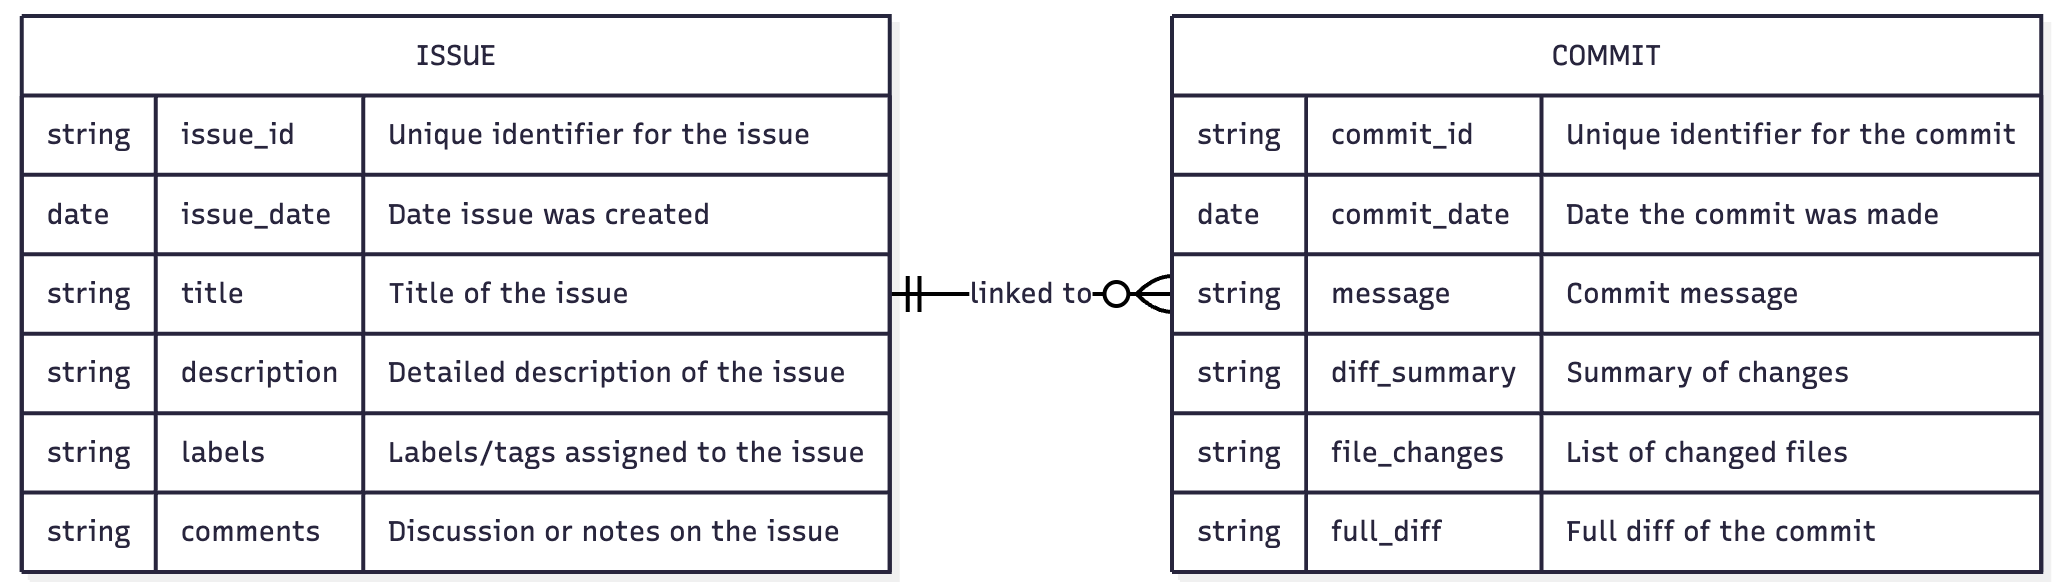
\includegraphics[width=0.98\textwidth]{Figures/er-issue-commit.png}
    \captionsetup{font={small,it},justification=centering}
    \caption{ER model for one-to-many relationship between issues and commits}
    \label{fig:er_issue_commit}
\end{figure}


As shown in Fig.~\ref{fig:er_issue_commit}, each \textit{Issue} entity can be linked to multiple \textit{Commit} entities, capturing the incremental nature of software development where complex issues are often resolved over several commits.


\subsubsection*{Disconnect Between Issue Trackers and Version Control Systems}

A significant challenge in this area arises from the separation between issue tracking systems (e.g., Bugzilla, GitHub) and version control systems (e.g. Mercurial)~\cite{r1,r2}. The lack of integration between the tools results in incomplete traceability hindering maintenance and analytics. Developers may manually include issue IDs in commit messages, but this practice is often inconsistent and error-prone~\cite{r16,r18}, reducing the ability to analyze software changes and understand the rationale behind them. To fill this gap, we present \textbf{LinkRank}, a learning-to-rank formulation for one-to-many issue-commit linking.\\

\noindent
The remainder of this paper is structured as follows. Section 3 reviews the related work. Section 5 introduces the proposed \emph{LinkRank} framework and its variant \textsc{LinkRank-C2I}, detailing the feature design, LambdaMART training, and selection strategies. Section-6 describes the experimental setup and Section-7 presents the results across multiple repositories.

% \bibliographystyle{IEEEtran}
% \bibliography{Reference_Cleaned_IEEE}


\section{Motivation}

\subsection{Agentic AI: a new paradigm for repository-scale automation}
Agentic AI enables models to act autonomously, plan complex tasks, and integrate tools/memory for long-term objectives. In software, these systems monitor development, analyze history, and perform tasks like finding fixes or triaging issues. Unlike simple prompt-driven LLMs, Agentic AI combines perception, retrieval, and iterative decision-making: forming hypotheses, validating them, and refining actions based on feedback. This significantly enhances automation for complex software engineering and bridges issue reporting with code changes.

% \noindent
% By prioritizing traceability, we provide a reliable foundation for higher-level agents (explainers, fix-suggesters, automatic integrators). Ultimately, robust, scalable traceability makes Agentic AI practical for maintenance, automation, and continuous quality assurance in real-world projects.


\subsection{The core problem: a gap in existing research}

Despite substantial prior work, from early heuristics and IR-based heuristics to modern machine learning and deep models, existing approaches predominantly assume a one-to-one mapping between an issue and a single commit~\cite{r17,r19,r20,r7}. This simplifying assumption overlooks three important realities:

    \begin{figure}[H]
        \centering
        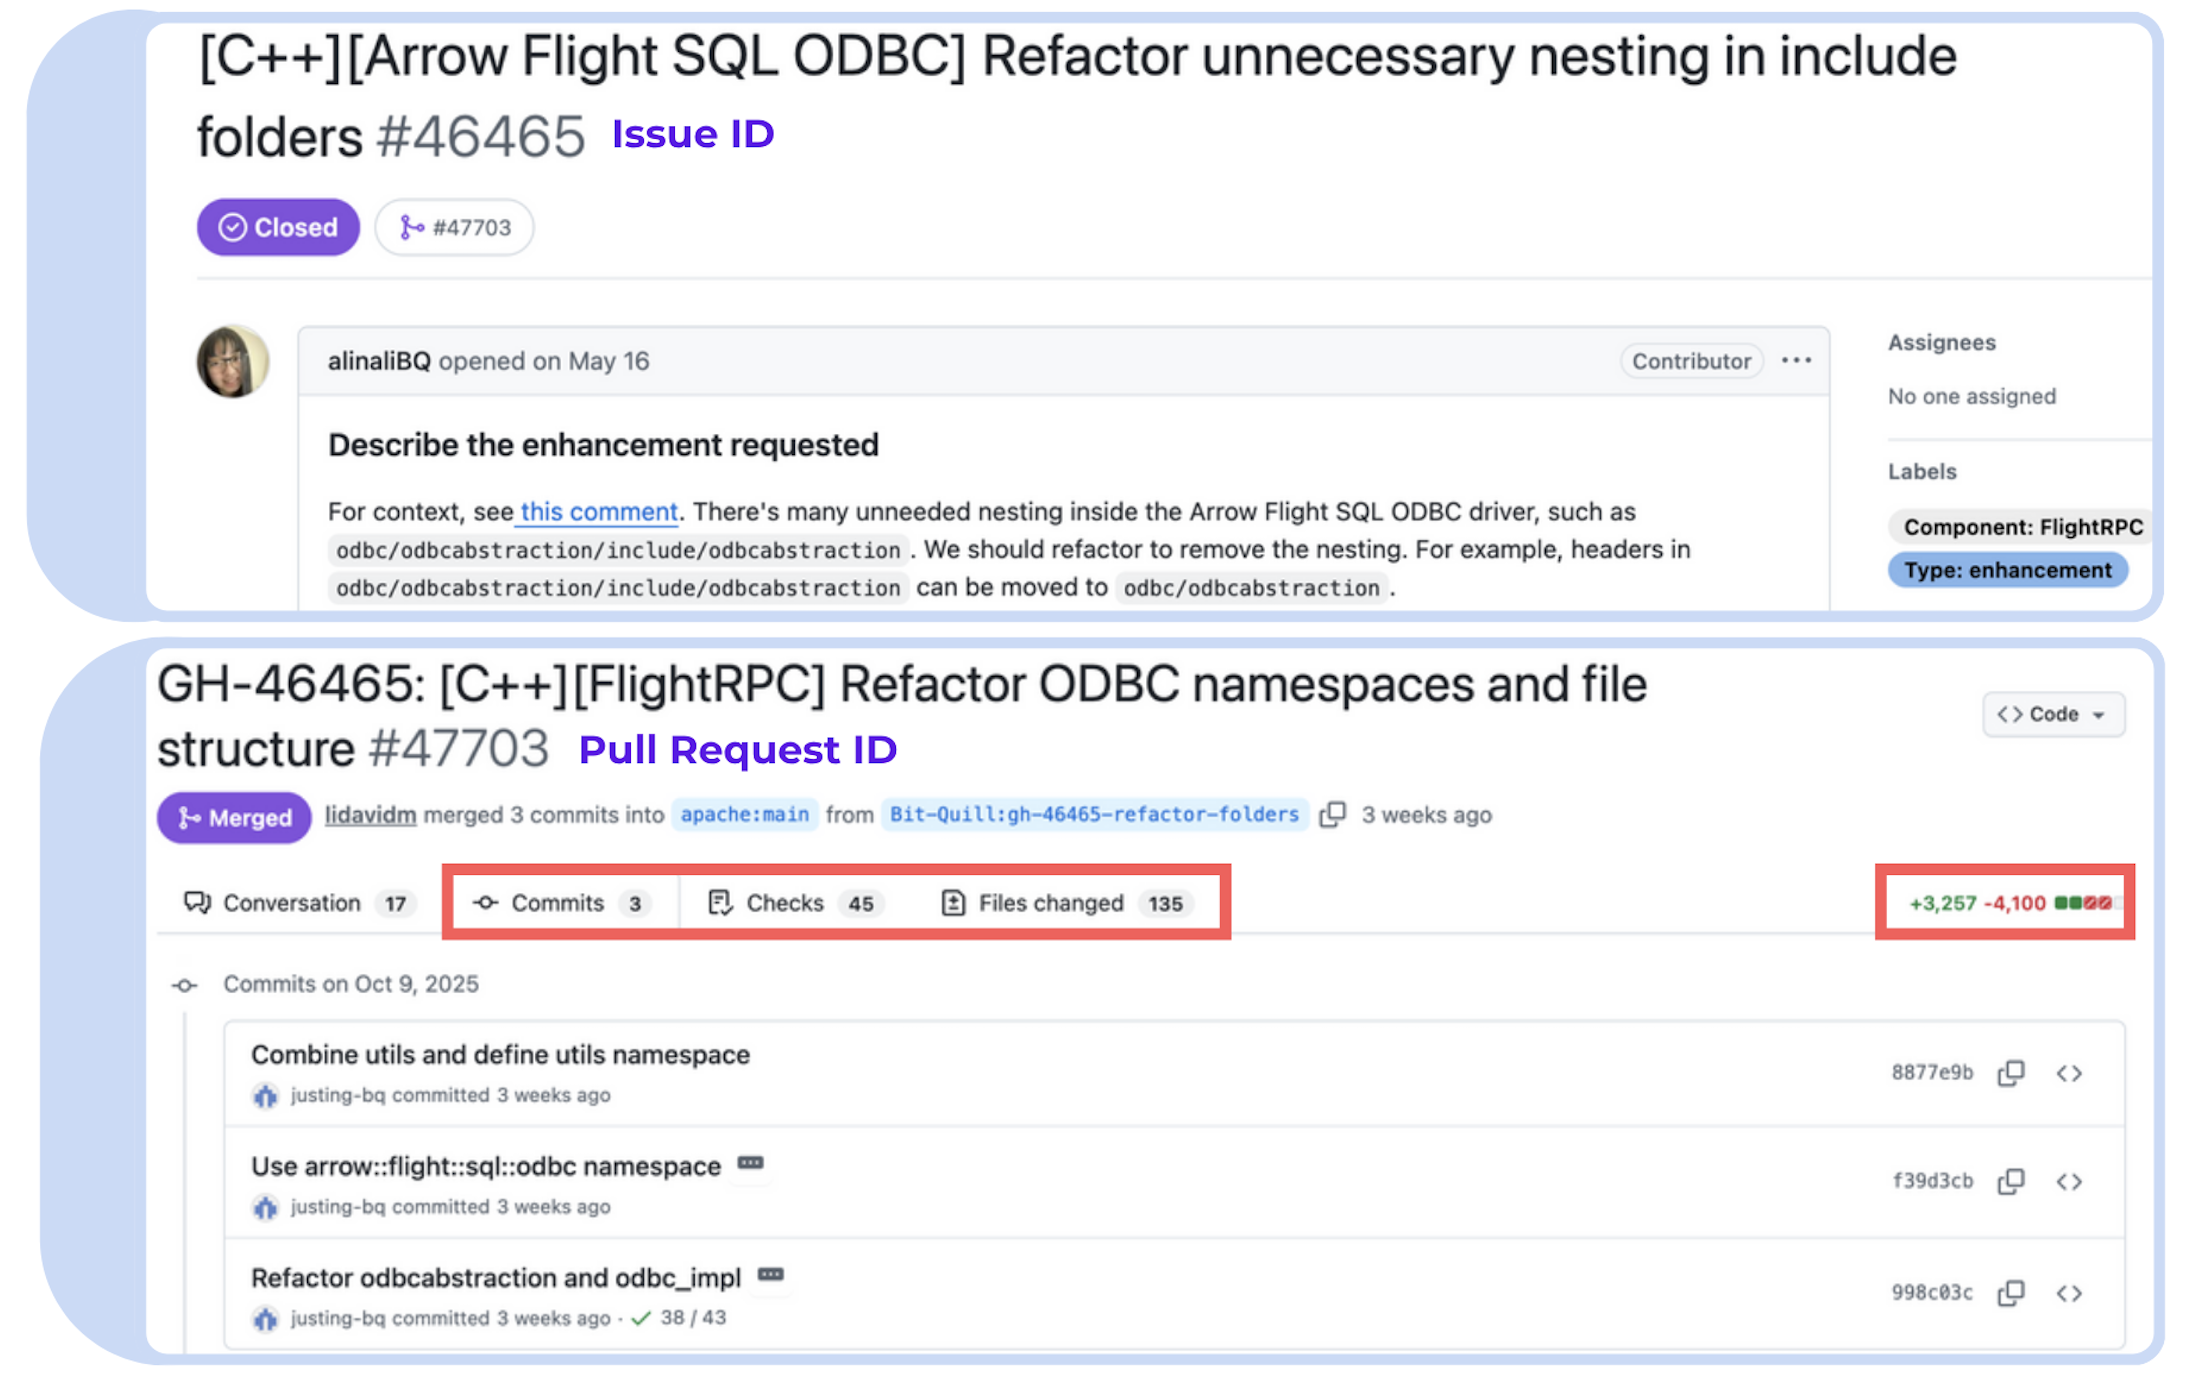
\includegraphics[width=0.9\textwidth]{Figures/issue-pr-demo-example.png}
        \captionsetup{font={small,it},justification=centering}
        \caption{A Practical Example of a One-to-Many Issue--Commit Relationship}
        \label{fig:issue_pr_demo_example}
    \end{figure}

\begin{enumerate}[a)]
	\item \textbf{Prevailing assumption: one-to-one issue--commit mappings.} Many automated methods are designed and evaluated under the assumption that each issue corresponds to a single commit. This simplifies modeling and evaluation but does not align with real development processes.
	
	\item \textbf{Prevalence of one-to-many relationships.} In practical development workflows a single issue, especially complex bugs or multi-step feature work, is often resolved through multiple commits (incremental fixes, follow-ups, or refactors)~\cite{r7,r17}. These one-to-many patterns are common in large and actively maintained projects. As shown in Fig.~\ref{fig:issue_pr_demo_example}, GitHub issue \textbf{\#46465}, titled ``[C++] [Arrow Flight SQL ODBC] Refactor unnecessary nesting in include folders,'' was resolved by a series of three commits bundled in pull request \textbf{\#47703}. The commits (in order of time, earliest first) are:
    \begin{itemize}
        \setlength\itemsep{0pt}
        \setlength\parskip{0pt}
        \setlength\topsep{0pt}
        \item \textit{Commit 1: Refactor odbcabstraction and odbc\_impl}
        \item \textit{Commit 2: Use \texttt{arrow::flight::sql::odbc} namespace}
        \item \textit{Commit 3: Combine utils and define utils namespace}
        \end{itemize}

    The scope of this multi-step refactoring and its volume is shown by the \texttt{Files changed} tab, which indicates these three commits modified a total of 135 files, along with 3,257 lines of additions and 4,100 lines of deletions. This example illustrates the complexity of real-world issue resolution, where multiple coordinated commits are necessary to fully address a single issue.

	\item \textbf{Failure to capture full resolution scope.} By ignoring one-to-many links, current traceability models fail to capture the full history and context of issue resolution. This fragmentation degrades downstream tasks such as debugging, historical analysis, and automated repair, because the complete set of commits that together implement a fix is not recovered~\cite{r7}.
\end{enumerate}


\subsection{The business impact: high software maintenance costs}

Traceability gaps have direct operational consequences. When links between issues and their resolving commits are missing or incomplete, engineers spend extra time searching, re-running tests, and performing manual code reviews to determine what changed and why. This increases mean time to repair and contributes to ongoing maintenance expenses across large codebases~\cite{r15,r16}. For organizations operating at scale, the cumulative cost of these inefficiencies is non-trivial and motivates automated, accurate linking solutions.\\

\noindent
Together, these observations motivate a targeted focus on one-to-many issue–commit recovery. Solving this foundational problem produces immediate practical benefits for maintenance and research and provides a reliable substrate for higher-level agentic systems that aim to autonomously link, explain, and resolve software issues.


\section{Objectives}

This literature review shows that, despite substantial advances in both traceability and agentic code-repair systems, the two areas remain largely disconnected. Traditional link-recovery approaches provide robust traceability but often lack explainability and automation; agentic systems (e.g., MAGIS) enable automated fixing but typically operate without explicit traceability grounding. Bridging these paradigms calls for a unified framework that combines interpretable trace links with automated repair capabilities.\\

\noindent
Accordingly, we propose a threefold objective for future research in agentic software maintenance:

\begin{enumerate}
    \item robust \textbf{issue--commit traceability} that explicitly models one-to-many relationships between issues and commits using a learning-to-rank approach; It also involves creating a comprehensive dataset containing one-to-many issue–commit pairs that captures these complex link structures for training and evaluation.
    \item \textbf{explainability mechanisms} that justify link predictions by citing the specific parts of an issue addressed by each commit in natural language; and
    \item \textbf{agentic automation for bug resolution} to propose and, where appropriate, implement fixes guided by traceability evidence and rationales generated by the explainability layer.
\end{enumerate}
\begin{center}
\begingroup
\setlength{\fboxsep}{6pt}% adjust padding as needed
\fbox{%
    \begin{minipage}{\linewidth}
        \textbf{Scope Statement:} This report focuses on and covers the major part of \emph{Task 1: issue--commit traceability} only ,  namely, the design, implementation, and evaluation of explainable, multi-commit issue–commit traceability. Explainability and multi-agent bug fixing frameworks are discussed as future work.
    \end{minipage}%
}
\endgroup
\end{center}

These objectives frame the rest of the report: designing the dataset and feature set, implementing the LinkRank ranking and selection pipeline, evaluating optional semantic features, and validating the approach with a rigorous per-issue protocol to demonstrate its practical benefits for one-to-many issue--commit traceability recovery.\\

\noindent
In the next section, we present \emph{LinkRank}, a learning-to-rank formulation designed specifically for one-to-many issue--commit linking. In LinkRank each issue is treated as a query and candidate commits are ranked using a compact, interpretable feature blend: lexical similarity (TF--IDF with SVD) and retrieval-focused signals (BM25). Ranking is learned with a LambdaMART model and selection uses an iterative pick--remove--renormalize policy. 








\section{Literature Review}

\subsection{Software Traceability and Automated Link Recovery}
Software traceability, the process of establishing and maintaining connections between related software artifacts, is fundamental to understanding, evolving, and maintaining complex software systems~[1],~[2]. It enables effective impact analysis~[3], assists in bug fixing and project management~[5], and is critical to ensuring safety in mission-critical domains~[4].  
A particularly important dimension of traceability is \emph{issue–commit linking}, which connects issues reported in tracking systems (such as Bugzilla~[9]) to the commits in version control systems (such as Git~[11]) that address them~[6]–[8].\\

While developers can manually reference issue identifiers within commit messages, this practice is inconsistent, leading to missing or incomplete links~[13]. Such gaps obscure the rationale behind code changes and increase maintenance costs~[14]–[16]. Consequently, establishing reliable automated links is vital for downstream research areas such as bug prediction~[17] and commit analysis~[18].  
Over the past two decades, automated approaches to issue–commit linking have evolved from early rule-based systems~[17],~[19],~[20], to classical machine-learning models~[21]–[25], and more recently to deep learning and transformer-based frameworks~[7],~[26]–[31] that capture deep semantic relationships between textual and code artifacts.

\subsection{Rule-Based and Heuristic Approaches}
Early attempts at automated link recovery relied on explicit rules and heuristics, mainly exploiting textual similarity between issue descriptions and commit messages.
\begin{itemize}
    \item \textbf{LINKSTER: Query-Based Manual Inspection} --- Bird \textit{et al.}~\cite{linkster} highlighted the tedious manual effort required to identify missing links and introduced \textbf{LINKSTER}, a tool that facilitated this process by providing query interfaces over issue and commit data. Although LINKSTER simplified retrieval, it relied heavily on manual inspection and lacked full automation.
    \item \textbf{ReLink: Early Automation using Textual Similarity} --- Wu \textit{et al.}~\cite{relink} developed \textbf{ReLink}, considered the first automated approach for recovering missing links through textual similarity. Treating issue reports and commit messages as plain text enabled feature extraction via token frequency and cosine similarity. However, its exclusive reliance on lexical overlap limited its ability to detect semantically related but lexically dissimilar pairs.
    \item \textbf{MLINK: Incorporating Structural (Source-Code) Information} --- Nguyen \textit{et al.}~\cite{mlink} introduced \textbf{MLINK}, extending ReLink by combining textual features with structural information from modified source code. By analyzing actual code changes, MLINK integrated linguistic and syntactic cues, significantly improving precision over purely text-based approaches.
    \item \textbf{RCLinker: Leveraging Generated Commit Messages} --- \textbf{RCLinker}~\cite{q3} addressed the problem of missing or poor-quality commit messages by incorporating automatically generated commit summaries from ChangeScribe~\cite{r27,r28}. By fusing generated and developer-written messages, RCLinker used a random-forest classifier to estimate the likelihood of a link, achieving higher accuracy than heuristic systems.
    \item \textbf{FRLink: Incorporating Non-Source Documents} --- \textbf{FRLink}~\cite{r56} broadened the analysis to include non-source artifacts such as documentation and build scripts that accompany commits. Through contextual filtering, FRLink captured additional signals ignored by purely source-centric methods, improving recall without compromising precision.
    \item \textbf{PULink: Positive-Unlabelled (PU) Learning} --- Recognizing that most unlinked pairs are not truly negative but unlabelled, \textbf{PULink}~\cite{q4} reframed the problem as a Positive-Unlabelled task. This perspective allowed better discrimination between true negatives and unlabeled examples, improving generalization and robustness.
    \item \textbf{HybridLinker: Fusing Textual and Non-Textual Classifiers} --- \textbf{HybridLinker}~\cite{q2} combined textual and structural classifiers using an ensemble model. A weighted fusion of predictions from both sources yielded higher precision and reduced computational overhead, illustrating the benefit of hybrid feature spaces in link recovery.
\end{itemize}

\subsection{Deep Learning and Transformer-Based Approaches}
Recent advances leverage deep neural networks and pre-trained transformers to model complex, non-linear semantic relationships between issues and commits.
\begin{itemize}
    \item \textbf{DeepLink: Code Knowledge Graphs} --- \textbf{DeepLink}~\cite{q1,rene3} was one of the first deep models for issue–commit recovery. It proposed a code knowledge-graph representation to preserve semantic information that is often lost in text-only or bag-of-words models, enabling deeper contextual understanding of commits and their associated issues.
    \item \textbf{T-BERT: Transfer Learning for Data Scarcity} --- \textbf{T-BERT}~\cite{rene4} adopted transfer learning to mitigate limited labeled data in software repositories. By fine-tuning BERT on issue–commit datasets, it achieved notable improvements over traditional machine-learning baselines with minimal domain-specific supervision.
    \item \textbf{BTLink: Dual-Encoder Fusion Architecture} --- \textbf{BTLink}~\cite{btlink} advanced transformer-based models through dual BERT encoders for issues and commits, merged via a fusion layer. This architecture enhanced cross-project adaptability and provided better semantic matching.
    \item \textbf{EALink: Knowledge Distillation and Contrastive Learning} --- \textbf{EALink}~\cite{ealink} focused on efficiency and representation quality through knowledge distillation and contrastive learning. It reduced model size while retaining high accuracy, addressing scalability issues in large repositories.
\end{itemize}

\subsection{Research Gap in Existing Link-Recovery Methods}
Despite these advances, most studies continue to model the problem as a \emph{one-to-one binary classification} task. In practice, software issues are often resolved across multiple commits, each addressing partial aspects such as refactoring, testing, or incremental fixes. Existing frameworks, including advanced transformer-based ones, fail to model these \emph{one-to-many relationships}, leading to incomplete traceability.  
Furthermore, current datasets and evaluation protocols assume a single best commit per issue, reinforcing this oversimplification. The absence of inter-commit relationship modeling also limits downstream tasks such as commit clustering, bug root-cause reasoning, and automated fix generation.  
Hence, there exists a critical gap: the need for a scalable, explainable, and automation-ready model that captures \textbf{multi-commit traceability} and \textbf{causal link reasoning}.

\subsection{Explainability in Software Engineering}
Explainability has emerged as a key pillar of modern software-engineering AI systems. Beyond generating predictions, models must justify their reasoning to support developer trust, auditing, and debugging.  
In the context of traceability, explainable models can articulate why a commit is linked to an issue, by citing specific textual or structural evidence, thereby bridging the gap between automated inference and human comprehension.  
Recent explainable approaches incorporate attention visualization, natural-language rationales, and code summarization to elucidate linking decisions. Such transparency is essential for integrating automated systems into collaborative software environments.

\subsection{Agentic AI for Software Automation}
\subsubsection*{Rise of Agentic AI}
Agentic AI marks a shift from static large-language-model (LLM) interfaces to autonomous, goal-driven agents capable of planning, acting, and reasoning over extended tasks. These agents possess memory, environmental awareness, and tool-use capabilities. In software engineering, this paradigm enables systems that can autonomously analyze repositories, generate code patches, perform testing, and iteratively improve solutions.\\

Practical, developer-facing systems also reflect this agentic trend. Tools such as GitHub Copilot, Anthropic's Claude (including Claude Code variants), Cursor, and Windsurf provide varying degrees of workspace-aware assistance. While not all of these systems are full multi-step autonomous agents, they illustrate how LLM-powered assistants are being embedded into IDEs and developer workflows, lowering the barrier to broader agentic automation in everyday software maintenance.

\subsubsection*{Multi-Agent Frameworks in Software Maintenance}
Multi-agent frameworks coordinate specialized agents to emulate collaborative developer workflows. By dividing responsibilities, such as task decomposition, code generation, review, and validation, these frameworks achieve scalability and robustness. They also naturally support feedback loops that approximate team-based software maintenance processes.

\subsubsection{MAGIS: Multi-Agent GitHub Issue Resolution}
\textbf{MAGIS}~\cite{magis} exemplifies the integration of LLM-based agents for end-to-end issue resolution. The framework comprises four primary agents:

\begin{itemize}
    \item \textbf{Manager Agent} -- Acts as the planner and coordinator: it decomposes a reported issue into concrete subtasks, prioritizes work, and assigns those tasks to a team of Developer agents.
    \item \textbf{Repository Custodian} -- Responsible for efficient context retrieval within large codebases: the custodian locates relevant files, functions, and hunks that pertain to the issue and prepares compact summaries for downstream agents.
    \item \textbf{Developer Agents} -- Implement and modify code in a structured, parallelizable workflow: developers generate candidate patches, apply targeted edits, and decompose complex modifications into smaller sub-operations (e.g., generate, refactor, adapt). 
    \item \textbf{QA Engineer Agent} -- Provides task-specific validation and feedback through reasoning and automated testing, paired with each Developer agent to ensure timely reviews. 
\end{itemize}

\begin{figure}[h!]
    \centering
    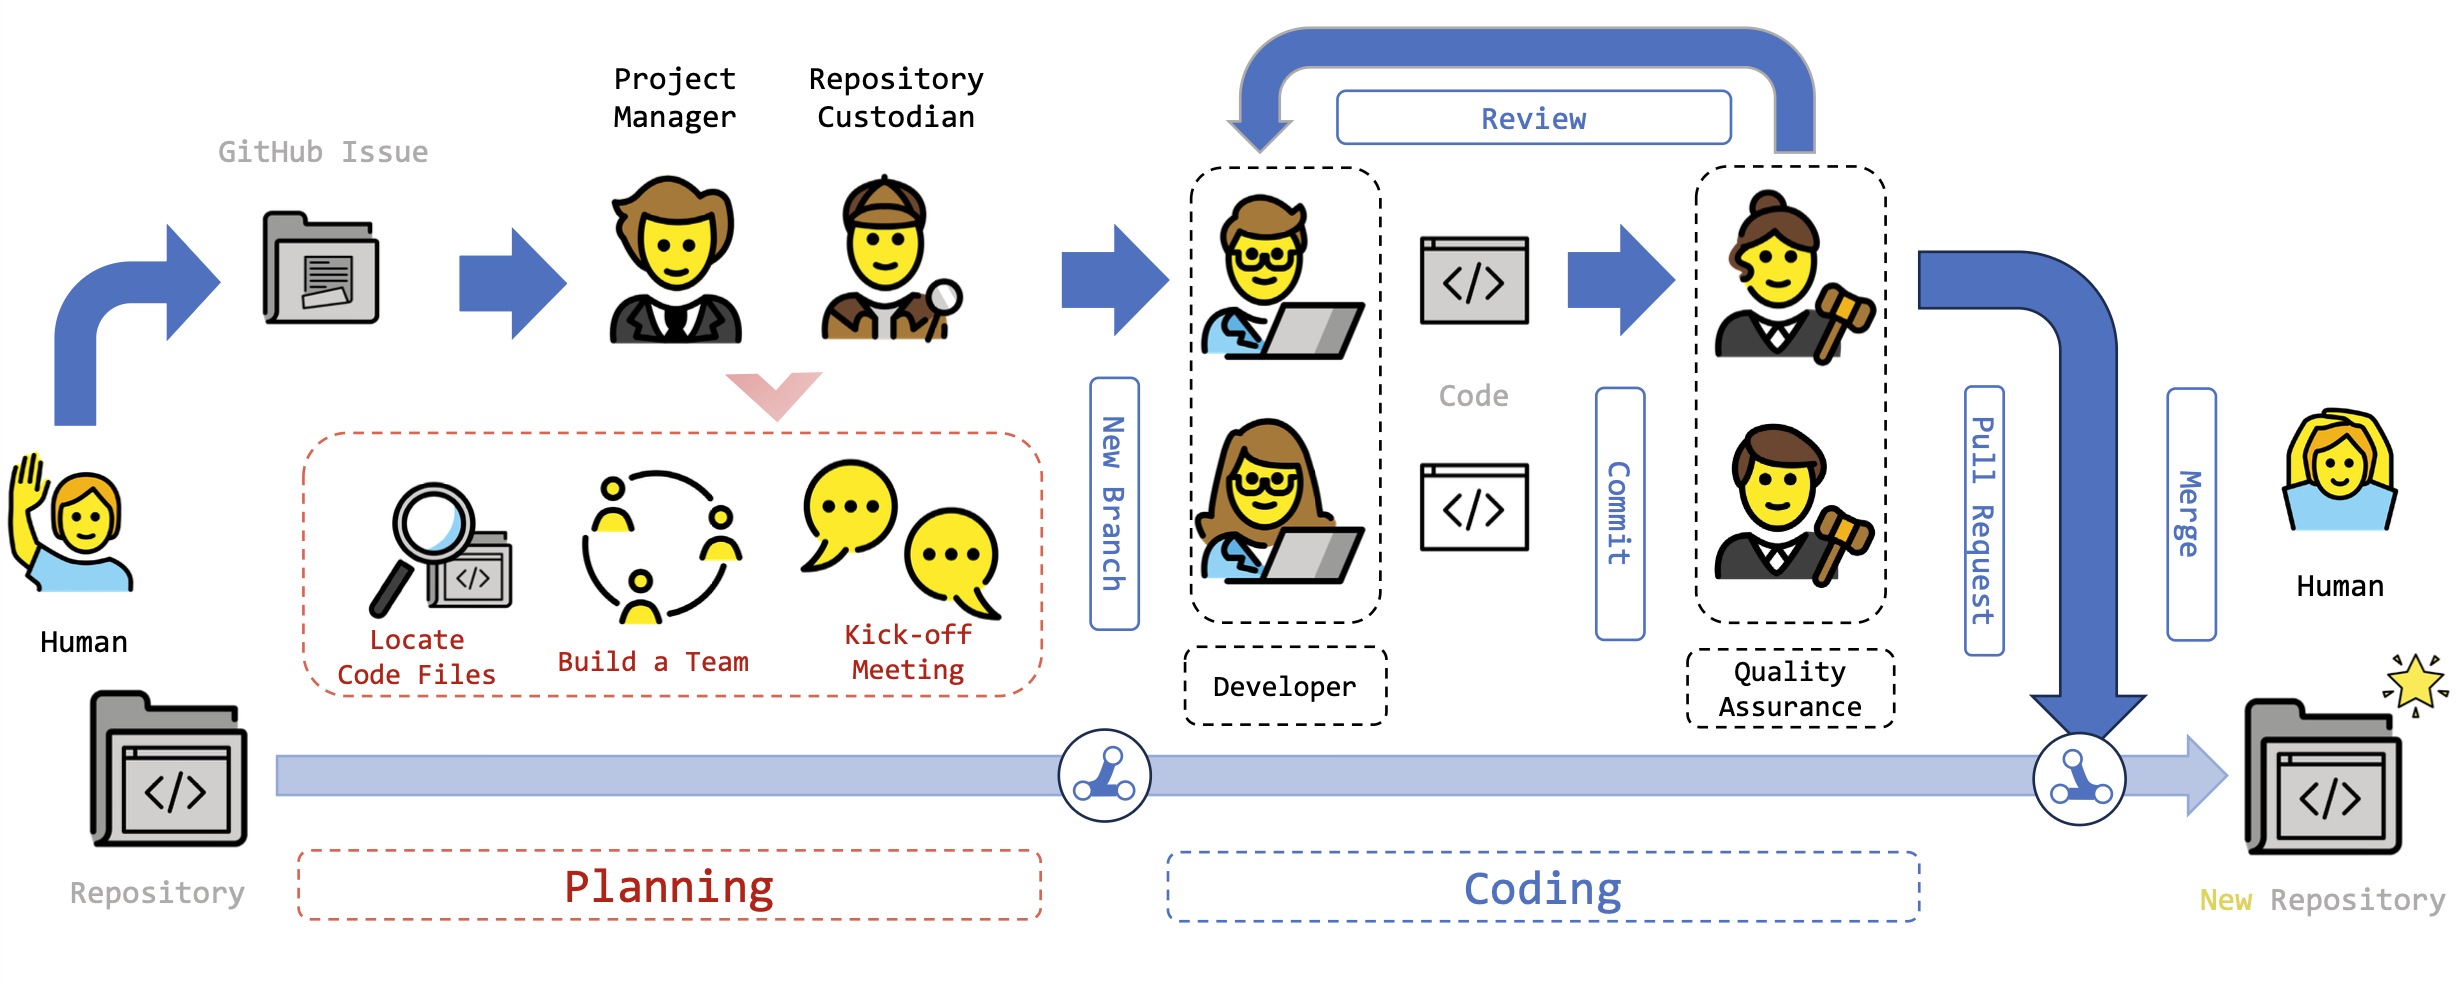
\includegraphics[width=0.88\textwidth]{figures/magis-architecture.png}
    \caption{Architecture of the MAGIS Multi-Agent Framework for GitHub Issue Resolution.}
    \label{fig:magis_architecture}
\end{figure}

MAGIS overcomes three major limitations in prior LLM-based repair systems:
(1) lack of fine-grained localization,  
(2) inability to reason about multi-file dependencies, and  
(3) absence of iterative validation.  
Evaluated on the SWE-Bench benchmark, MAGIS achieved an accuracy of 13.94\%, representing an eight-fold improvement over baseline GPT-4 performance.

\subsubsection{ExpeRepair: Dual-Memory Enhanced LLM-based Repo-Level Program Repair}

ExpeRepair~\cite{mu2025expeRepair} is a repository-level program repair framework that augments LLM-based repair agents with a dual-memory architecture. Repair work is performed by a Program Repair Module (Test Agent + Patch Agent) which iteratively generates reproduction tests, proposes patches, and validates candidate fixes. After each repair attempt, ExpeRepair records the trajectory (tests, patches, execution feedback) and extracts reusable examples and summarized strategies for future in-context use.

\begin{figure}[H]
    \centering
    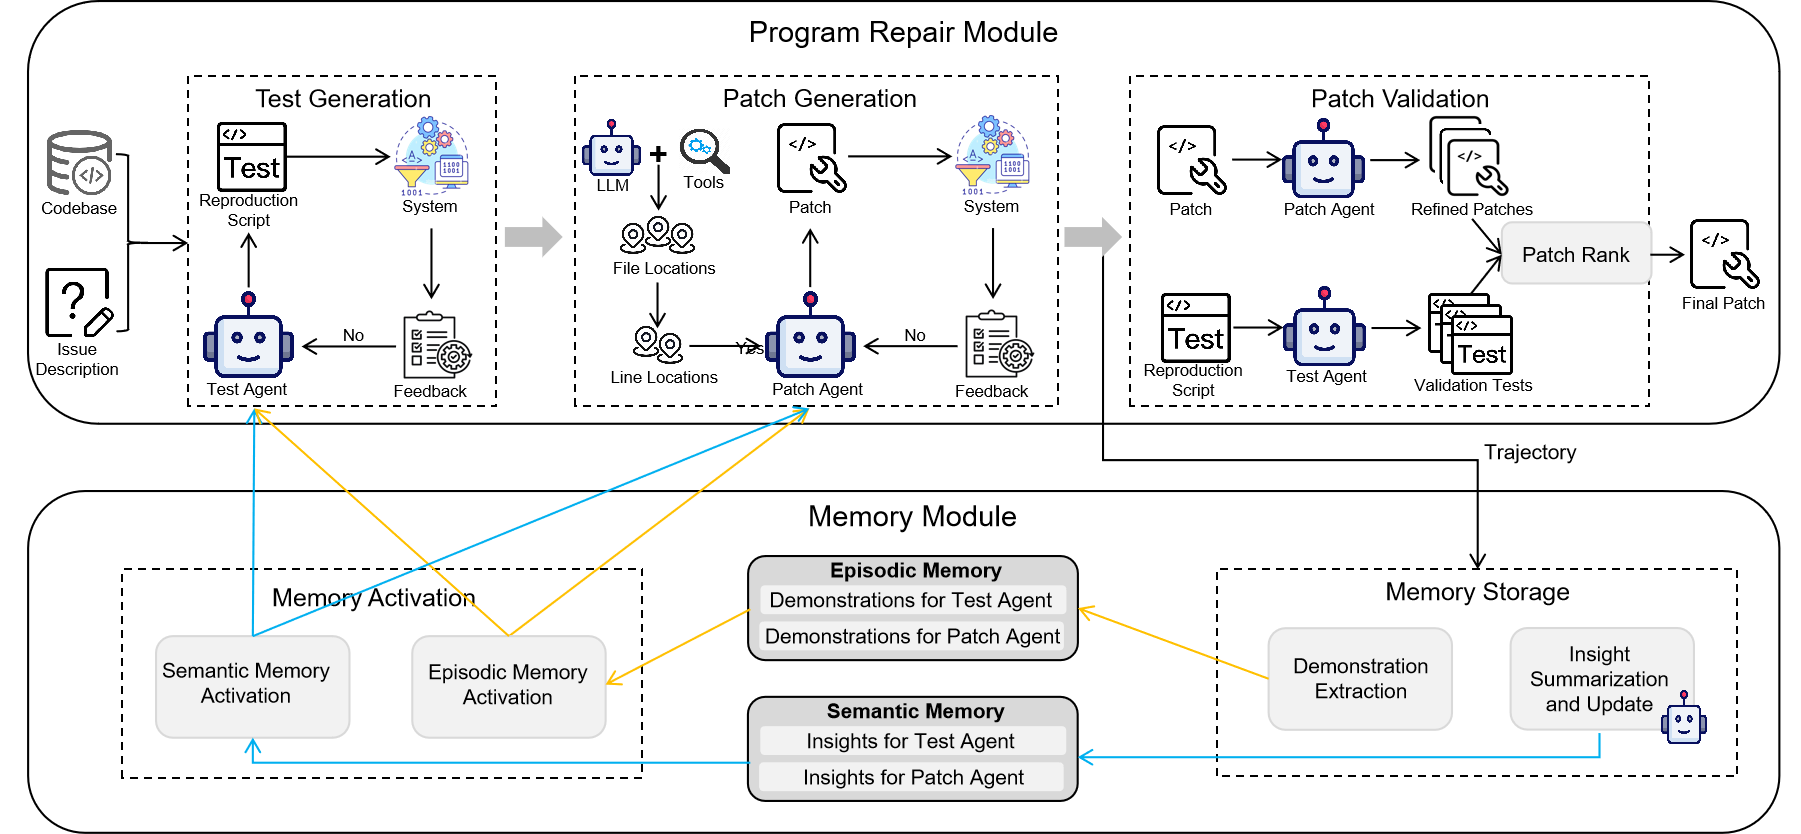
\includegraphics[width=0.82\textwidth]{figures/experepair-overview.png}
    \caption{Architecture of the ExpeRepair: Dual-Memory Enhanced LLM-based Program Repair.}
    \label{fig:expeRepair_architecture}
\end{figure}

As shown in Fig.~\ref{fig:expeRepair_architecture}, ExpeRepair maintains two complementary memory stores:  \emph{episodic memory} and \emph{semantic memory}. After the program repair module processes a new issue, the memory module collects the complete repair trajectory, which consists of all detailed artifacts associated with that specific repair instance, including the issue description, reproduction scripts, candidate patches, and the test execution results before and after each patch is applied.\\

\noindent
Rather than relying on expensive parameter updates, ExpeRepair uses a two-phase workflow: an initial seed phase to populate memories from a curated set of issues, and an inference phase where the agents retrieve top-$k$ demonstrations and applicable insights to enrich prompts and guide generation. This experience-driven prompting enables faster warm-starts, more robust test generation and patching (by reusing prior handling of similar failures), and progressive improvement in repair success rates without model fine-tuning. It achieves state-of-the-art performance among open-source methods, resolving 47.7\% of issues when using Claude 3.5 Sonnet V2.

% \subsection{Proposed Work}


\newpage
\section{Summary of Work Done}


Our approach is organized into four phases. The complete workflow is illustrated in Figure~\ref{fig:approach}. The workflow comprises the following four main phases / steps:
\begin{enumerate}
    \setlength{\itemsep}{2pt}
    \setlength{\parskip}{0pt}
    \item Dataset construction
    \item Feature representations
    \item Learning-to-rank (LambdaMART)
    \item Selection strategies
\end{enumerate}

\begin{figure}[h!]
    \centering
    \includegraphics[width=0.98\textwidth]{figures/App.png}
    \caption{Overall workflow of the proposed LINKRANK framework}
    \label{fig:approach}
\end{figure}




\subsection{Phase I: Dataset construction process}

% Brief: this subsection describes how repositories, issues, and commits were selected and filtered to build a one-to-many issue--commit dataset, and summarizes dataset statistics.

The dataset for this study was constructed using GitHub’s API to extract issue--commit pairs from multiple repositories. GitHub imposes a rate limit of 5,000 requests per hour per authenticated user, making data extraction a time-consuming process~\cite{GitHubAPI}. To ensure that the dataset captured realistic one-to-many relationships, we specifically filtered issues that were linked to at least two and at most six commits. Identifying repositories that contained a sufficiently large number of such issues proved challenging, as many projects either had too few one-to-many cases or exhibited extreme imbalance. Therefore, we selected repositories with a sufficient number of issues satisfying the 2–6 commit criterion. 

\begin{table*}[htbp]
\centering
\caption{Statistics of selected GitHub repositories used for dataset construction.}
% Reduce vertical density and horizontal padding so the table fits within page margins
\renewcommand{\arraystretch}{1.2}
\setlength{\tabcolsep}{4pt}
\label{stats}
\scriptsize
% Constrain the project name column to allow line-wrapping and avoid overflow
\begin{tabular}{p{2.5cm}ccccccc}
\hline
\multirow{2}{*}{\textbf{Project Name}} & 
\multirow{2}{*}{\textbf{Commits}} & 
\multirow{2}{*}{\textbf{Issues}} &
\multicolumn{5}{c}{\textbf{Number of Issues with N Commits}} \\ \cline{4-8}
 &  &  & \textbf{Two Commits} & \textbf{Three Commits} & \textbf{Four Commits} & \textbf{Five Commits} & \textbf{Six Commits} \\ \hline
Apache/Beam        & 3104 & 486 & 206 & 110 & 81 & 54 & 31 \\
Apache/Datafusion  & 3534 & 496 & 135 & 132 & 95 & 79 & 52 \\
Apache/Superset    & 3136 & 498 & 230 & 105 & 65 & 56 & 41 \\
Apache/Mxnet       & 1216 & 187 & 69 & 49 & 36 & 19 & 14 \\
Apache/Dubbo       & 1205 & 201 & 97 & 46 & 22 & 20 & 16 \\
Apache/Iceberg     & 1750 & 257 & 97 & 57 & 36 & 39 & 26 \\
Kubernetes         & 2948 & 483 & 238 & 102 & 66 & 43 & 31 \\
grpc               & 2162 & 486 & 131 & 84 & 51 & 34 & 28 \\
TensorFlow         & 2719 & 408 & 167 & 86 & 69 & 45 & 35 \\
PyTorch            & 748  & 125 & 51 & 45 & 14 & 9 & 6 \\ \hline
\end{tabular}
\end{table*}

The overall dataset statistics are summarized in Table~\ref{stats}, providing a detailed view of the scale and distribution of the collected data. This systematic filtering process ensured both the scalability of the dataset and its fidelity to real-world development practices.

\begin{table*}[htbp]
\centering
\caption{Programming languages in the selected GitHub repositories and their total stars.}
\label{tab:repo-langs}
\scriptsize
\renewcommand{\arraystretch}{1.3}
\setlength{\tabcolsep}{10pt}
\begin{tabular}{l l c c c c c c c}
\hline
	\textbf{Project} & \textbf{Owner} & \textbf{Stars} & \textbf{Java} & \textbf{Python} & \textbf{Rust} & \textbf{C++} & \textbf{Go} & \textbf{JS/TS} \\ \hline
Beam               & Apache     & 8.3k  & \ding{51} & \ding{51} & \ding{55} & \ding{55} & \ding{55} & \ding{55} \\
DataFusion         & Apache     & 7.7k  & \ding{55} & \ding{55} & \ding{51} & \ding{55} & \ding{55} & \ding{55} \\
Superset           & Apache     & 67.8k & \ding{55} & \ding{51} & \ding{55} & \ding{55} & \ding{55} & \ding{51} \\
MXNet              & Apache     & 20.8k & \ding{55} & \ding{51} & \ding{55} & \ding{51} & \ding{55} & \ding{55} \\
Dubbo              & Apache     & 41.3k & \ding{51} & \ding{55} & \ding{55} & \ding{55} & \ding{55} & \ding{55} \\
Iceberg            & Apache     & 7.9k  & \ding{51} & \ding{55} & \ding{55} & \ding{55} & \ding{55} & \ding{55} \\
Kubernetes         & Kubernetes & 117k  & \ding{55} & \ding{55} & \ding{55} & \ding{55} & \ding{51} & \ding{55} \\
gRPC (grpc)        & grpc       & 43.6k & \ding{55} & \ding{55} & \ding{55} & \ding{55} & \ding{51} & \ding{55} \\
TensorFlow         & TensorFlow & 191k  & \ding{55} & \ding{51} & \ding{55} & \ding{51} & \ding{55} & \ding{55} \\
PyTorch            & PyTorch    & 93.2k & \ding{55} & \ding{51} & \ding{55} & \ding{51} & \ding{55} & \ding{55} \\ \hline
\end{tabular}

\vspace{3pt}
\footnotesize{
    \ding{51} = present / primary language \quad\quad \ding{55} = not present / minor traces}
\end{table*}

Table~\ref{tab:repo-langs} summarizes the primary programming languages used in each selected repository, highlighting the diversity of languages (Java, Python, Rust, C++, Go, JavaScript/TypeScript) represented in our dataset. This variety ensures that our approach is evaluated across different coding styles and practices, enhancing its generalizability. The languages were identified using GitHub's Linguist tool, which analyzes the repository contents to determine the primary programming languages used.


\subsubsection*{False Link Generation}

% Brief: this subsubsection explains our PR-aware strategy for creating realistic negative samples (false links) that balance positives per-issue while avoiding semantic overlap.

Constructing a reliable set of false links is critical for evaluating issue-commit link recovery models, as it enables a more accurate assessment of the models' ability to distinguish between correctly linked and mismatched issue-commit pairs. However, previous works have often faced challenges in generating false links, which may compromise the quality of the datasets used for model evaluation. Thus, we propose a novel approach for generating false links that addresses these challenges.

\noindent
Several existing studies have relied on simplistic strategies for generating false links, which can lead to inaccuracies. For example, BTLink \cite{btlink} and DeepLink \cite{q1} generated false links by randomly pairing issues and commits from separate projects or unrelated time periods. This approach risks introducing semantically related links that were mistakenly labeled as false, as code changes made in close time proximity or in related repositories may still be connected to the same issue. Similarly, HERMES \cite{hermes} and EALink \cite{ealink} created false links using time-based sampling techniques, where issues and commits were paired if they were not linked within a specific time frame. However, this method overlooks the possibility that complex issue resolutions may involve multiple commits spread over extended periods, potentially leading to the inclusion of valid links being mislabeled as false. Additionally, T-BERT \cite{tbert} generated a large number of false links without verifying their semantic separation from true links, leading to datasets where negative pairs may still be contextually relevant, thus reducing the reliability of the ground truth.\\


% \begin{figure*}[htbp] % t=top, b=bottom, h=here, H=exact (needs \usepackage{float})
%   \centering
%   \includegraphics[width=\linewidth]{qwqwqwqwq.png}
%   \caption{Overall workflow of the proposed \textsc{LinkRank} framework, illustrating its four main phases: Data preparation, Feature Representations, Learning-to-Rank, and Selection Strategies.}
%   \label{approach}
% \end{figure*}



% \begin{figure*}[t] % t=top, b=bottom, h=here, H=exact (needs \usepackage{float})
%   \centering
%   \includegraphics[width=\linewidth]{App.png}
%   \caption{Overall workflow of the proposed \textsc{LinkRank} framework, illustrating its four main phases: Data preparation, Feature Representations, Learning-to-Rank, and Selection Strategies.}
%   \label{approach}
% \end{figure*}

To address these limitations, we adopt a Pull Request (PR)-aware strategy for generating false links. We first identify valid PRs that satisfy our condition of having between 2 and 6 commits. For each valid PR $p$, we denote its corresponding issue as $i_p$ and the set of associated commits as $C_p = \{c_1, c_2, \dots, c_m\}$, where $2 \leq m \leq 6$. The set of true links is therefore defined as $T = \{(i_p, c_j) \mid p \in \mathcal{P}_{\text{valid}},\; c_j \in C_p\}$.\\

Next, we consider PRs that do not satisfy the 2--6 commit constraint, denoted as $\mathcal{P}_{\text{invalid}}$. From these PRs, we construct a pool of unrelated commits:
\[
C_{\text{invalid}} = \bigcup_{p \in \mathcal{P}_{\text{invalid}}} C_p.
\]

For each valid issue $i_p$ with $m = |C_p|$ true commits, we generate an equal number of false links by randomly sampling $m$ unrelated commits from $C_{\text{invalid}}$. This ensures that the number of false links matches the number of true links on a per-issue basis: $F_p = \{(i_p, c_r) \mid c_r \sim \text{Uniform}(C_{\text{invalid}}), \; |F_p| = m \}$.\\

\noindent
Finally, the dataset is formed by combining true and false links, i.e., $D = T \cup \bigcup_{p \in \mathcal{P}_{\text{valid}}} F_p$.\\

\noindent
This construction guarantees balance between positive and negative samples for each issue, while keeping the false links realistic and repository-aware. The PR-aware false link generation strategy minimizes the risk of semantic overlap between true and false links, thereby enhancing the reliability of the dataset for evaluating issue-commit link recovery models.


\subsection{Phase II: Feature Representations}

% Brief: this subsection describes the feature channels (lexical, retrieval-based, semantic) used to encode issue--commit pairs into compact vectors for ranking.

To effectively model the one-to-many issue--commit linking problem, each candidate pair $(i,c)$ is encoded into a feature vector $x_{ic}$ that captures complementary dimensions of similarity. Rather than relying on a single view of the data, we combine lexical, retrieval-based, and optional semantic features, enabling the model to distinguish true links from superficially similar but incorrect ones. 

\subsubsection{Lexical Similarity (TF--IDF + SVD).}
% Brief: explains the TF--IDF + truncated SVD lexical channel and the cosine similarity feature used to quantify lexical alignment between issues and commits.
For the lexical perspective, we employ Term Frequency--Inverse Document Frequency (TF--IDF), a well-established method in information retrieval for quantifying the salience of terms relative to a corpus. The TF component reflects how often a term appears in a document (issue or commit), while the IDF component down-weights terms that are frequent across the whole corpus and up-weights rarer, more discriminative terms. To capture latent topics and reduce dimensionality, we apply truncated Singular Value Decomposition (SVD), yielding compact dense representations. The cosine similarity between an issue vector $v_i$ and a commit vector $v_c$ is then
\[
f_{\text{text}}(i,c) = \frac{\langle v_i, v_c \rangle}{\|v_i\|\cdot \|v_c\|},
\]
where $\langle v_i, v_c \rangle$ is the dot product and $\|v_i\|$, $\|v_c\|$ are vector norms. High values indicate strong lexical alignment, while the SVD projection smooths sparsity and captures latent semantics beyond exact token overlap.

\subsubsection{BM25 Matching.}
% Brief: describes BM25 as a query-focused retrieval score that models term importance and document length for issue-as-query vs. commit-as-document matching.
While TF--IDF provides global representations, retrieval often benefits from query-focused matching. BM25 \cite{bm25}, a probabilistic ranking function widely used in search engines, is particularly effective here. It improves upon TF--IDF by modeling diminishing returns for repeated term occurrences and by normalizing document length, thus avoiding bias toward longer commit messages. Treating the issue text as a query and the commit text as a document, BM25 yields
\[
f_{\text{bm25}}(i,c) = \sum_{t \in i} \text{IDF}(t) \cdot 
\frac{f(t,c)\cdot (k_1+1)}{f(t,c) + k_1\!\cdot\!\left(1 - b + b \cdot \tfrac{|c|}{\text{avgdl}}\right)}.
\]
Here, $\text{IDF}(t)$ emphasizes rare terms, $f(t,c)$ counts term occurrences in commit $c$, $|c|$ is the commit length, $\text{avgdl}$ is the average commit length in the \emph{training} corpus, $k_1$ controls frequency saturation, and $b$ tunes length normalization. In this way, BM25 captures how well a commit matches an issue when the issue is interpreted as a retrieval query.



\subsubsection{Semantic Similarity (CodeBERT).}
% Brief: outlines the optional CodeBERT-based semantic channel which provides vector embeddings to capture paraphrases and code-aware context beyond lexical signals.
In addition to lexical and retrieval features, we include a complementary semantic signal from CodeBERT \cite{codebert}, a transformer model pre-trained on natural language and code. We compute mean-pooled embeddings $\phi(i)$ and $\phi(c)$ for the issue and commit, L2-normalize them, and score with cosine similarity:
\[
f_{\text{sem}}(i,c) = \cos\big(\phi(i), \phi(c)\big).
\]
This semantic channel complements TF--IDF and BM25 by capturing paraphrases and code-aware context (e.g., terse messages or alternate phrasings). Importantly, our ablations show that the model remains strong \emph{without} CodeBERT; adding it primarily improves robustness in cases where wording diverges or context is sparse.






\subsection{Phase III: Learning-to-Rank with LambdaMART}
% Brief: describes training a LambdaMART ranker on the extracted feature vectors (grouped by issue) to directly optimize ranking metrics for one-to-many recovery.
To transform the extracted feature representations into an effective linking model, we employ \textit{LambdaMART} \cite{lambda}, a gradient boosted decision tree algorithm specifically designed for ranking tasks. Unlike conventional classification methods that predict binary labels, LambdaMART directly optimizes ranking-based metrics such as the Normalized Discounted Cumulative Gain (NDCG), making it particularly well suited for the one-to-many issue--commit linking problem.


The central idea is to model relative preferences between commits for each issue. Training data are grouped by issue, ensuring that the model does not learn absolute scores across unrelated issues, but instead learns how to order candidate commits within each issue context (Algorithm~\ref{algo_1}). Given the feature vector $x_{ic}$ for an issue--commit pair $(i,c)$, LambdaMART learns a non-linear scoring function $\mathcal{R}$ through gradient-boosted regression trees. The output of the model is a ranking score:
\[
s(i,c) = \mathcal{R}(x_{ic}),
\]
where higher scores indicate stronger likelihood of a true issue--commit link.

This formulation offers two key benefits. First, it allows the model to focus directly on ranking quality rather than classification accuracy, which is crucial in settings where each issue may be linked to multiple commits. Second, tree-based boosting naturally captures complex, non-linear feature interactions (e.g., when lexical similarity is high but BM25 matching is weak, or when semantic similarity diverges), yielding a more discriminative and flexible ranking function. At inference time, we score a pool of candidate commits for each issue and then apply an \emph{iterative} selection rule: we pick the current top commit, remove it from the pool, recompute per-issue normalization $\tilde{s}(i,c)$ (min--max scaled) and the updated $s_{\max}$, and repeat until the stopping rule is met. Thus, LambdaMART forms the foundation of our \textsc{LinkRank} framework, enabling robust recovery of one-to-many issue--commit links.


\subsection{Phase IV: Selection Strategies}
% Brief: explains iterative post-processing policies (Known-K oracle and two Unknown-K thresholding rules) that convert per-issue rankings into final one-to-many link sets.
Once the ranking scores are obtained, the final prediction set $\widehat{\mathcal{C}}(i)$ for each issue $i$ must be constructed. We follow an \emph{iterative pick--remove--renormalize} procedure: at each step, select according to the chosen policy, remove the selected commit from the pool, and recompute per-issue normalization (min--max $\tilde{s}$) and the current $s_{\max}$ before the next step. We distinguish between two cases:  

\paragraph{Known-K} In this case, we assume that the true number of commits $K$ associated with issue $i$ is known (an oracle setting). We iteratively take the top-ranked commit, remove it, renormalize scores, and continue until exactly $K$ commits have been selected. Although impractical in deployment (since the true $K$ is rarely available), this strategy serves as an important upper bound to evaluate the performance of our framework. 

\paragraph{Unknown-K} In this case, the number of commits linked to each issue is not known beforehand. This makes the task considerably harder, as the system must automatically determine not only which commits to link, but also how many. To address this challenge, we introduce two threshold-based strategies that adapt selection to the relative or absolute quality of ranking scores:
\begin{itemize}
    \item \textit{Absolute Thresholding (ABS):} At each iteration, after renormalization, link any commit whose normalized score $\tilde{s}(i,c)$ exceeds a fixed threshold $\tau$; remove selected commits and repeat until no remaining candidate exceeds $\tau$. This imposes a global cutoff across issues.
    \item \textit{Relative Thresholding (REL):} At each iteration, with the current top score $s_{\max}(i)$, link any commit satisfying $s(i,c) \ge \gamma \cdot s_{\max}(i)$; remove selected commits, recompute $s_{\max}(i)$, and continue until no remaining candidate satisfies the $\gamma$ criterion. This adapts to per-issue score scales.
\end{itemize}

Together, these strategies allow us to contrast oracle-based performance (Known-K) with more realistic scenarios (Unknown-K). The ABS rule emphasizes global calibration, while the REL rule emphasizes local adaptivity, and both operate within the same iterative pick--remove--renormalize loop, making them well-suited for the one-to-many linking problem.



\begin{algorithm}[htbp]
\caption{LinkRank }
\label{algo_1}
\begin{algorithmic}[1]
\STATE \textbf{Input:} Issues $\mathcal{I}$, commits $\mathcal{C}$, labeled pairs $\mathcal{D}$
\STATE \textbf{Output:} Predicted links $\{\widehat{\mathcal{C}}(i)\}_{i\in\mathcal{I}}$
\STATE Build corpora $S_{\mathcal{I}}, S_{\mathcal{C}}$; compute TF--IDF{+}SVD and BM25 features; \textit{(optional) }CodeBERT features
\FORALL{$(i,c,y)\in\mathcal{D}$}
  \STATE Build feature $x_{i,c}$ 
\ENDFOR
\STATE Train LambdaMART ranker $\mathcal{R}$ grouping by \textbf{Issue ID}
\FORALL{$i\in\mathcal{I}$}
  \FORALL{$c\in\mathcal{C}$}
    \STATE $s(i,c)\gets \mathcal{R}(x_{i,c})$
  \ENDFOR
  \STATE Compute per-issue normalized scores $\tilde{s}(i,c)$ via min--max; let $s_{\max}(i)\gets \max_{c}s(i,c)$
  \STATE \textit{Iterative selection:} repeat
  \STATE \hspace{0.6cm}Pick $c^\star \in \arg\max_{c} s(i,c)$ if admissible by the chosen policy
  \STATE \hspace{0.6cm}Add $c^\star$ to $\widehat{\mathcal{C}}(i)$; remove $c^\star$ from the candidate pool
  \STATE \hspace{0.6cm}Recompute $\tilde{s}(i,c)$ (min--max) and update $s_{\max}(i)$
  \STATE until stopping criterion is met
  \STATE \textbf{Selection policies:}
  \STATE \hspace{0.6cm}\textbf{Known-$K$:} select exactly the top $K$ commits
  \STATE \hspace{0.6cm}\textbf{Unknown-$K$ (ABS):} select all $c$ with $\tilde{s}(i,c)\ge \tau$
  \STATE \hspace{0.6cm}\textbf{Unknown-$K$ (REL):} select all $c$ with $s(i,c)\ge \gamma \cdot s_{\max}(i)$
\ENDFOR
\end{algorithmic}
\end{algorithm}


\subsection{Phase V: Bidirectional Variant: LinkRank-C2I}

In addition to our primary framework, \textsc{LinkRank}, which adopts an issue-centric perspective, we also experimented with a variant called \textsc{LinkRank-C2I} (commit$\rightarrow$issue). The motivation is to provide a complementary view by reversing the linking perspective. Since issue--commit relationships are inherently bidirectional, examining the task from the commit side lets us study whether different linking dynamics emerge when commits are treated as queries, and it further enables a consistency check between both directions, as detailed in Algorithm~\ref{algo_2}.



\textbf{Step 1: Commit-to-Issue Retrieval.}\ \
Each commit $c \in \mathcal{C}$ is treated as a query and issues $i \in \mathcal{I}$ are candidates. Feature representations (TF--IDF+SVD, BM25, and optional CodeBERT) are computed exactly as in \textsc{LinkRank}, but tuples are grouped by \textbf{commit} for training. A LambdaMART ranker $\mathcal{R}_{A2}$ learns to score candidate issues:
\[
s_{A2}(c,i) = \mathcal{R}_{A2}(x_{c,i}),
\]
where $x_{c,i}$ is the feature vector for commit $c$ and issue $i$. To restrict the search space, we retain only the top-$K$ issues per commit:
\[
\mathcal{S}(c) = \mathrm{Top}\text{-}K \{\, i \in \mathcal{I} \mid s_{A2}(c,i) \,\}.
\]
(Optionally, a BM25 guard can expand the candidate set with a few high-recall issues per commit.)

\textbf{Step 2: Issue-to-Commit Validation.}\ \
We then reintroduce the issue-centric view of \textsc{LinkRank}. For each issue $i$, we restrict its candidate pool to those commits that shortlisted $i$ in Step~1:
\[
\mathcal{P}(i) = \{\, c \in \mathcal{C} \mid i \in \mathcal{S}(c) \,\}.
\]
The Issue-to-Commit ranker $\mathcal{R}_{A1}$ (trained by grouping tuples \textbf{by issue}) is applied to this reduced pool, producing refined scores:
\[
s(i,c) = \mathcal{R}_{A1}(x_{i,c}), \quad c \in \mathcal{P}(i).
\]
This cross-directional gating enforces agreement between the commit$\rightarrow$issue and issue$\rightarrow$commit views.

% typically reducing false positives while preserving recall.

\textbf{Selection Strategies.}\ \
We use the same policies as in \textsc{LinkRank} (Known-$K$, Unknown-$K$ ABS, and Unknown-$K$ REL) with the same \emph{iterative} procedure: pick the current best commit for $i$, remove it from $\mathcal{P}(i)$, recompute per-issue normalization (min--max $\tilde{s}$) and the updated $s_{\max}(i)$, and continue until the stopping rule is met.

In summary, \textsc{LinkRank-C2I} complements the primary approach by enforcing bidirectional consistency, typically reducing false positives while preserving recall.




\begin{algorithm}[htbp]
\caption{LinkRank-C2I}
\label{algo_2}
\begin{algorithmic}[1]
\STATE \textbf{Input:} Issues $\mathcal{I}$, commits $\mathcal{C}$, labeled pairs $\mathcal{D}$
\STATE \textbf{Output:} Predicted links $\{\widehat{\mathcal{C}}(i)\}_{i\in\mathcal{I}}$
\STATE Build corpora $S_{\mathcal{I}}, S_{\mathcal{C}}$; compute TF--IDF{+}SVD and BM25 features; \textit{(optional) }CodeBERT features
\FORALL{$(i,c,y)\in\mathcal{D}$}
  \STATE Build feature $x_{i,c}$ 
\ENDFOR
\STATE Train commit$\rightarrow$issue ranker $\mathcal{R}_{\text{C2I}}$ (group by \textbf{Commit ID}) and issue$\rightarrow$commit ranker $\mathcal{R}_{\text{I2C}}$ (group by \textbf{Issue ID})

\vspace{0.25em}
\STATE \textbf{Stage 1 — Commit$\rightarrow$Issues (shortlist)}
\FORALL{$c\in\mathcal{C}$}
  \STATE $s_{\text{C2I}}(c,i)\gets \mathcal{R}_{\text{C2I}}(x_{c,i})$ for all $i\in\mathcal{I}$
  \STATE shortlist $\mathcal{S}(c)\gets$ top-$K$ issues ranked by $s_{\text{C2I}}$
\ENDFOR

\vspace{0.25em}
\STATE \textbf{Stage 2 — Issue$\rightarrow$Commits (final selection)}
\FORALL{$i\in\mathcal{I}$}
  \STATE pool $\mathcal{P}(i)\gets \{\,c\in\mathcal{C}: i\in\mathcal{S}(c)\,\}$
  \STATE $s(i,c)\gets \mathcal{R}_{\text{I2C}}(x_{i,c})$ for $c\in\mathcal{P}(i)$
  \STATE sort by $s$; let $s_{\max}$ be top; compute per-issue $\tilde{s}$ (min--max)
  \STATE \textit{Iterative rule}: after each pick, remove it from $\mathcal{P}(i)$ and recompute per-issue normalization
  \STATE \textbf{Selection strategies:} apply Known-$K$, Unknown-$K$ ABS, or Unknown-$K$ REL as in Algorithm~\ref{algo_1}
\ENDFOR
\end{algorithmic}
\end{algorithm}
\section{Experimental Setup}

\subsection{Experimental Settings}
All experiments were conducted on a dedicated server equipped with an \textit{NVIDIA RTX 4500 Ada Generation GPU} with \textit{24 GB} of VRAM, running CUDA version 12.5 and driver version \textit{555.42.06}. The system further consisted of a multi-core Intel CPU and 64 GB of RAM, running Ubuntu Linux (64-bit). Our implementation is based on Python 3.10 with \texttt{scikit-learn} and \texttt{xgboost} for learning-to-rank, and HuggingFace \texttt{transformers} for optional CodeBERT embeddings. To ensure reliable evaluation, we adopted a 5-fold stratified cross-validation strategy~\cite{stone1974cross}. For each repository, the labeled data was divided into five folds, with four folds used for training and the remaining fold reserved for testing. All reported results represent the average performance across the five folds, providing a balanced and consistent protocol for assessing model effectiveness across projects.


% Training and inference were executed in mixed-precision mode where applicable to maximize efficiency. Unless otherwise specified, all reported results are averaged over three independent runs with identical hyperparameters to account for variance.





% \subsection{Evaluation Metrics}


% In a one-to-many relationship, an issue may be associated with multiple commits. Therefore, evaluating each issue-commit pair independently does not reflect the model's effectiveness in recovering complete commit sets for issues. To address this, we adopt an issue-wise evaluation strategy, where each \textit{Issue\_ID} (represents an issue with a set of commits) is treated as a unit. For every issue, we compute the confusion matrix components, True Positives ($TP$), False Positives ($FP$), False Negatives ($FN$), and True Negatives ($TN$), based on the set of predicted and actual linked commits. These values are then used to calculate Precision, Recall, and F1-score per issue. Finally, we report the average of these scores across all issues to provide an overall measure of model performance.

% \paragraph{Precision ($Precision_{one-to-many}$)}

% Precision in the one-to-many setting measures the proportion of correctly predicted commits among all commits predicted to be linked to an issue.

% \[
% \text{Precision}_{\text{one-to-many}}^{(i)} = \frac{TP_i}{TP_i + FP_i}
% \]

% Where:
% \begin{itemize}
%     \item $TP_i$: Number of true positives for issue $i$ (correctly predicted linked commits).
%     \item $FP_i$: Number of false positives for issue $i$ (commits incorrectly predicted as linked).
% \end{itemize}

% The overall precision is computed as the average across all issues:
% \[
% \text{Precision}_{\text{one-to-many}} = \frac{1}{|I|} \sum_{i \in I} \text{Precision}_{\text{one-to-many}}^{(i)}
% \]

% \paragraph{Recall ($Recall_{one-to-many}$)}

% Recall measures the ability of the model to retrieve all relevant commits for an issue.

% \[
% \text{Recall}_{\text{one-to-many}}^{(i)} = \frac{TP_i}{TP_i + FN_i}
% \]

% Where:
% \begin{itemize}
%     \item $FN_i$: Number of false negatives for issue $i$ (linked commits not predicted).
% \end{itemize}

% The average recall across all issues is:
% \[
% \text{Recall}_{\text{one-to-many}} = \frac{1}{|I|} \sum_{i \in I} \text{Recall}_{\text{one-to-many}}^{(i)}
% \]

% \paragraph{F1-Score ($F1_{one-to-many}$)}

% The F1-score balances precision and recall for each issue:

% \[
% \text{F1}_{\text{one-to-many}}^{(i)} = \frac{2 \cdot \text{Precision}^{(i)} \cdot \text{Recall}^{(i)}}{\text{Precision}^{(i)} + \text{Recall}^{(i)}}
% \]

% And the final F1-score is computed by averaging:
% \[
% \text{F1}_{\text{one-to-many}} = \frac{1}{|I|} \sum_{i \in I} \text{F1}_{\text{one-to-many}}^{(i)}
% \]

\subsection{Evaluation Metrics}

In a one-to-many relationship, an issue may be linked to multiple commits. Evaluating each issue--commit pair independently fails to capture how effectively a model recovers the complete set of commits for an issue. To address this, we adopt an \emph{issue-wise evaluation} strategy: each issue $i$ (identified by its \textit{Issue\_ID}) is treated as a single evaluation unit. For every issue, we compute the confusion matrix components—True Positives ($TP_i$), False Positives ($FP_i$), and False Negatives ($FN_i$)—from which we derive Precision, Recall, and F1-score. The final results are obtained via \emph{macro-averaging}, ensuring that all issues contribute equally regardless of their number of linked commits.

\paragraph{Precision and Recall.}
Precision quantifies correctness, while Recall measures completeness of retrieved commits for each issue:
\[
\text{Precision}^{(i)} = \frac{TP_i}{TP_i + FP_i}, \qquad
\text{Recall}^{(i)} = \frac{TP_i}{TP_i + FN_i}.
\]
The overall scores are macro-averaged across all issues:
\[
\text{Precision} = \frac{1}{|I|}\sum_{i \in I}\text{Precision}^{(i)}, \qquad
\text{Recall} = \frac{1}{|I|}\sum_{i \in I}\text{Recall}^{(i)}.
\]

\paragraph{General F$_\beta$-Score.}
The F$_\beta$-score provides a weighted harmonic mean of Precision and Recall, allowing control over their relative importance through the parameter $\beta$:
\[
\text{F}_{\beta}^{(i)} = (1+\beta^2)\frac{\text{Precision}^{(i)} \cdot \text{Recall}^{(i)}}{(\beta^2 \cdot \text{Precision}^{(i)}) + \text{Recall}^{(i)}}.
\]

\paragraph{F1-Score and Its Choice.}
For $\beta = 1$, the F$_1$-score simplifies to:
\[
\text{F1}^{(i)} = \frac{2 \cdot \text{Precision}^{(i)} \cdot \text{Recall}^{(i)}}{\text{Precision}^{(i)} + \text{Recall}^{(i)}}, \qquad
\text{F1} = \frac{1}{|I|}\sum_{i \in I}\text{F1}^{(i)}.
\]

We choose the F1-score because it provides a balanced measure of performance when both false positives (over-linking commits to an issue) and false negatives (missing true links) are equally important. In the issue--commit linking context, over-predicting leads to noisy traceability, while under-predicting omits valid relationships—thus, F1 offers a fair trade-off between precision and recall, capturing the model’s overall linkage accuracy.



% \paragraph{Jaccard Similarity.}
% In addition to precision, recall, and F-score, we also evaluate performance using the Jaccard coefficient, which provides a stricter measure of set-level similarity. For each issue $i$, let $C(i)$ denote the set of ground-truth linked commits and $\widehat{C}(i)$ the set of predicted commits. The Jaccard index is defined as:
% \[
% J(i) = \frac{|C(i) \cap \widehat{C}(i)|}{|C(i) \cup \widehat{C}(i)|}.
% \]

% Unlike pairwise metrics that consider links independently, Jaccard directly measures the overlap between the predicted and actual commit sets. This makes it particularly suitable for one-to-many linking, where recovering the complete set of commits associated with an issue is essential. For example, if an issue is linked to four commits and the model predicts three of them correctly but adds one incorrect commit, precision and recall may appear high, but the Jaccard score will penalize the discrepancy by considering the entire set overlap.  \\

% \noindent
% By averaging $J(i)$ across all issues, we obtain a macro-level Jaccard score that reflects how well the model captures issue–commit sets in their entirety. This provides complementary insights beyond conventional precision and recall, highlighting the framework’s ability to achieve holistic traceability rather than partial correctness.


\subsection{Training and Inference Costs}

We conducted a comparative analysis of training and testing times across our approaches and the baseline models to answer the question:
\emph{How do LinkRank and LinkRank-C2I perform in terms of computational efficiency compared to existing baselines while maintaining high predictive accuracy?}\\

Figure~\ref{fig:time} presents efficiency (x-axis, in minutes, log scale) together with effectiveness (y-axis, F-score). Each line connects test (left dot) and train (right dot) times, while the y-axis annotates the corresponding F-scores. This visualization highlights the balance between computational cost and predictive performance. The results show that our LinkRank variants achieve strong predictive performance while remaining significantly more lightweight. For instance, LinkRank and LinkRank-C2I complete training within 30--40 minutes and testing within 5--7 minutes, yet yield F-scores above 83. In contrast, baselines such as DeepLink and EALink consume far more computational resources (160--225 minutes of training and 10--15 minutes of inference) while producing substantially lower accuracy.\\

\begin{figure}[htbp]
	\centering
	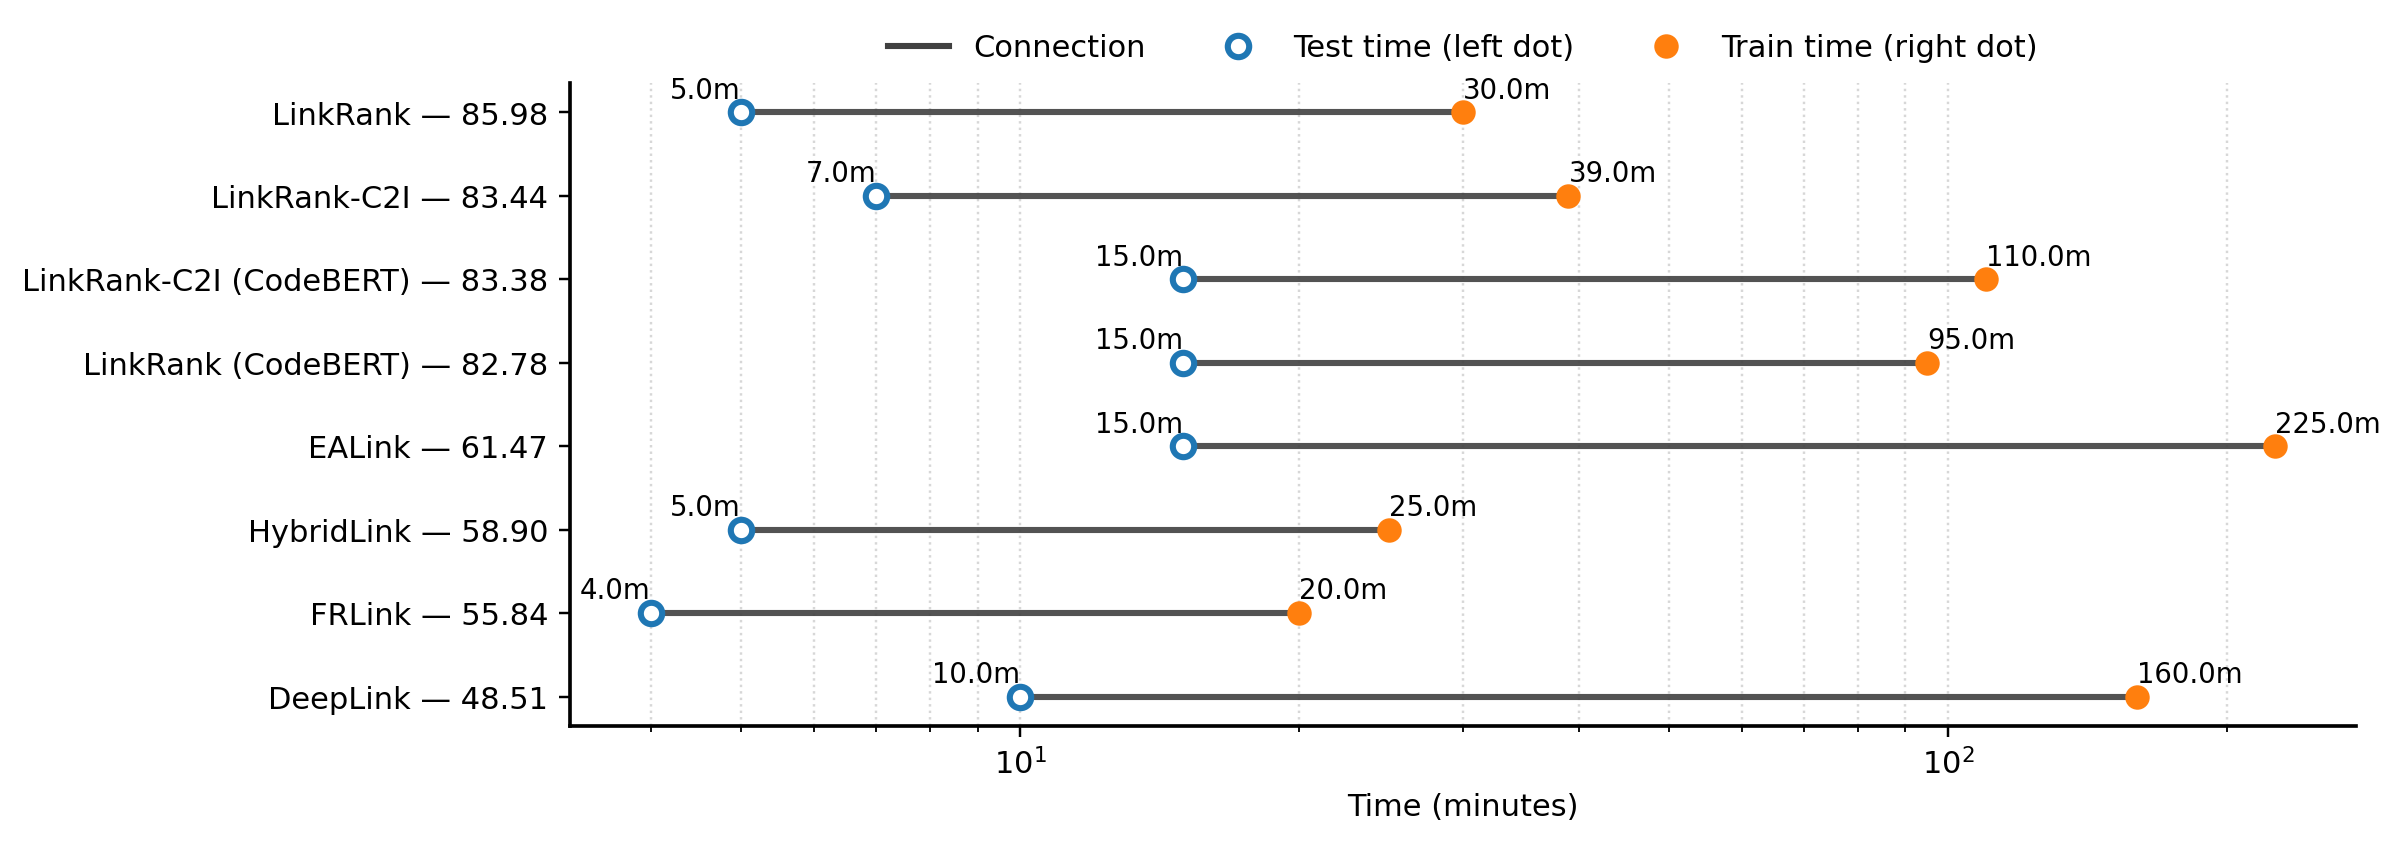
\includegraphics[width=\linewidth]{Figures/time.png}
	\caption{Training and inference time comparison of LinkRank, LinkRank-C2I, and baselines. }
	\label{fig:time}
\end{figure}

A key observation is that adding CodeBERT embeddings increases both training and testing costs by $3$--$4\times$ (e.g., 95--110 minutes of training), but delivers only marginal improvements in F-score. This highlights that the core design of LinkRank is already well suited for the largely pattern-matching nature of issue--commit recovery.





\section{Results}

We evaluate our proposed approaches, LinkRank and LinkRank-C2I, on the ten repositories described in Table~\ref{stats}. We compare their performance against several baselines across multiple metrics.

% \noindent\textbf{\large\textit{RQ1.} How do \textsc{LinkRank} and \textsc{LinkRank-C2I} compare against existing baselines?}

\subsection{Evaluation of LinkRank and LinkRank-C2I Against Baselines}

Table~\ref{rq3} presents the average performance across ten repositories, comparing our approaches with four representative baselines: EALink, HybridLink, FRLink, and DeepLink. The results clearly demonstrate that both LinkRank and LinkRank-C2I achieve substantially higher precision, recall, and F-score than all baselines under both Known-$K$ and Unknown-$K$ regimes.


\begin{table}[htbp]
\centering
\caption{Performance (in \%) comparison of LinkRank, LinkRank-C2I, and baselines. }
\subcaption*{These values are averaged across all datasets.}
\renewcommand{\arraystretch}{1.2}
\label{rq3}
\scriptsize
\begin{tabular}{llccc}
\toprule
\multicolumn{2}{c}{\textit{\textbf{Models}}} & \textit{\textbf{Precision}} & \textit{\textbf{Recall}} & \textit{\textbf{F-score}} \\
\midrule

\multirow{3}{*}{LinkRank} 
 & Known-K     & 93.05 & 93.05 & 93.05 \\
 & No-K - ABS  & 87.04 & 92.72 & 88.80 \\
 & No-K - REL  & 83.99 & 89.92 & 85.98 \\
\midrule

\multirow{3}{*}{LinkRank - C2I} 
 & Known-K     & 92.11 & 92.11 & 92.11 \\
 & No-K - ABS  & 84.61 & 93.16 & 87.45 \\
 & No-K - REL  & 85.83 & 83.92 & 83.44 \\
\midrule

% \multirow{3}{*}{LinkRank (CodeBERT)} 
%  & Known-K     & 91.93 & 91.93 & 91.93 \\
%  & No-K - ABS  & 86.75 & 93.48 & 88.95 \\
%  & No-K - REL  & 86.52 & 82.26 & 82.78 \\
% \midrule

% \multirow{3}{*}{LinkRank - C2I (CodeBERT)} 
%  & Known-K     & 92.14 & 92.14 & 92.14 \\
%  & No-K - ABS  & 85.86 & 92.65 & 88.04 \\
%  & No-K - REL  & 85.38 & 84.39 & 83.38 \\
% \midrule

\multirow{4}{*}{Baseline} 
 & EALINK\cite{ealink}     & 57.67 & 71.73 & 61.47 \\
 & HybridLink\cite{q2}  & 61.70 & 61.70 & 58.90 \\
 & FRLink\cite{r56}      & 46.43 & 73.85 & 55.84 \\
 & DeepLink\cite{q1}   & 49.58 & 51.422 & 48.51 \\
\bottomrule
\end{tabular}
\end{table}

Under the oracle \textit{Known-$K$} setting, LinkRank achieves an F-score of 93.05\%, closely followed by LinkRank-C2I at 92.11\%. These values are substantially higher than the best-performing baseline, EALink, which records only 61.47\%. In the more realistic \textit{Unknown-$K$} scenarios, our approaches continue to perform strongly. With ABS thresholding, LinkRank attains an F-score of 88.80\% and LinkRank-C2I achieves 87.45\%, while the baselines remain in the 48\%--61\% range. Under REL thresholding, LinkRank records 85.98\% and LinkRank-C2I achieves 83.44, again well above all baselines.\\

\textbf{Takeaway:} Across evaluation regimes, both LinkRank and LinkRank-C2I consistently outperform prior baselines by large margins, often exceeding them by 25--35 points in F-score. These results demonstrate that our learning-to-rank formulation is robust, generalizable, and establishes a new state of the art for one-to-many issue--commit link recovery. The weaker performance of baseline models can be attributed to their design: as discussed in the related work, existing approaches were primarily developed for one-to-one linking and treat the problem as a binary classification task, making them not well adapted to capture the complexity of one-to-many relations.



% Under the oracle \textbf{Known-$K$} setting, LinkRank reaches an average F-score of 91.91, while LinkRank-C2I attains 87.90. These scores are markedly higher than the best baseline, EALink, which achieves only 61.47 F-score. More importantly, in the more realistic \textbf{Unknown-$K$} scenarios, our models continue to dominate. For instance, under ABS thresholding, LinkRank achieves an average F-score of 86.82 and LinkRank-C2I achieves 84.24, compared to baseline values that remain in the 48--61 range. Under REL thresholding, LinkRank-C2I achieves an average F-score of 91.42, highlighting that bidirectional refinement can be highly effective in practice.

% \textbf{Takeaway.} Averaged across ten diverse repositories, both LinkRank and LinkRank-C2I deliver large, consistent gains over prior baselines, often exceeding them by 25--35 points in F-score. This establishes that our learning-to-rank formulation is not only robust and generalizable but also sets a new performance bar for one-to-many issue--commit link recovery.



% \textit{RQ2: How effective are LinkRank and its variant  LinkRank-C2I in recovering one-to-many issue--commit links?}

\subsection{Effectiveness of LinkRank and LinkRank-C2I for One-to-Many Recovery}

Table~\ref{rq2} reports results for both approaches under three selection regimes. As expected, \textit{Known-$K$} yields high scores across datasets, but it assumes oracle knowledge of the true number of commits per issue and is therefore not a realistic deployment setting. We thus focus our analysis on the \textit{Unknown-$K$} strategies (ABS and REL), which reflect practical use.\\

\begin{table*}[htbp]
\centering
\caption{Performance (in \%) of LinkRank and LinkRank-C2I} 
\subcaption*{Across 10 datasets under three regimes: Known-K, and Unknown-K with ABS and REL.}
\renewcommand{\arraystretch}{1.3}
\label{rq2}
\begin{tabular}{@{}llcccccc@{}}
\toprule
\multirow{2}{*}{\textbf{Dataset}} & \multirow{2}{*}{\textbf{Variations}} & \multicolumn{3}{c}{\textbf{LinkRank}} & \multicolumn{3}{c}{\textbf{LinkRank-C2I}} \\
\cmidrule(lr){3-5} \cmidrule(lr){6-8}
 &  & \textbf{Precision} & \textbf{Recall} & \textbf{F-score} & \textbf{Precision} & \textbf{Recall} & \textbf{F-score} \\
\midrule

\multirow{3}{*}{Apache/Beam}
 & Known K         & 91.29 & 91.29 & 91.29 & 90.35 & 90.32 & 90.33 \\
 & Unknown-K (ABS) & 84.67 & 89.92 & 86.04 & 83.24 & 90.63 & 85.59 \\
 & Unknown-K (REL) & 78.15 & 86.69 & 81.10 & 81.59 & 79.11 & 78.58 \\
\midrule

\multirow{3}{*}{Apache/Datafusion}
 & Known K         & 93.01 & 93.01 & 93.01 & 91.06 & 91.06 & 91.06 \\
 & Unknown-K (ABS) & 84.38 & 93.22 & 87.46 & 83.99 & 92.52 & 86.86 \\
 & Unknown-K (REL) & 82.16 & 88.72 & 84.09 & 83.50 & 81.52 & 80.89 \\
\midrule

\multirow{3}{*}{Apache/Superset}
 & Known K         & 95.04 & 95.04 & 95.04 & 91.89 & 91.89 & 91.89 \\
 & Unknown-K (ABS) & 90.57 & 93.67 & 91.35 & 82.52 & 91.65 & 85.28 \\
 & Unknown-K (REL) & 87.04 & 90.26 & 87.92 & 86.71 & 83.34 & 83.82 \\
\midrule

\multirow{3}{*}{Apache/Mxnet}
 & Known K         & 92.01 & 92.01 & 92.01 & 94.31 & 94.31 & 94.31 \\
 & Unknown-K (ABS) & 86.79 & 92.79 & 89.14 & 86.43 & 94.10 & 88.98 \\
 & Unknown-K (REL) & 85.93 & 88.73 & 86.63 & 89.45 & 88.38 & 88.08 \\
\midrule

\multirow{3}{*}{Apache/Dubbo}
 & Known K         & 92.72 & 92.72 & 92.72 & 91.42 & 91.42 & 91.42 \\
 & Unknown-K (ABS) & 87.31 & 93.15 & 89.23 & 76.00 & 95.42 & 83.54 \\
 & Unknown-K (REL) & 83.17 & 91.09 & 86.11 & 85.90 & 88.18 & 85.79 \\
\midrule

\multirow{3}{*}{Apache/Iceberg}
 & Known K         & 94.22 & 94.22 & 94.22 & 94.56 & 94.56 & 94.56 \\
 & Unknown-K (ABS) & 86.81 & 94.02 & 89.52 & 91.96 & 93.55 & 91.97 \\
 & Unknown-K (REL) & 87.93 & 91.41 & 89.22 & 88.07 & 85.04 & 85.40 \\
\midrule

\multirow{3}{*}{Kubernetes}
 & Known K         & 89.03 & 89.03 & 89.03 & 93.66 & 93.66 & 93.66 \\
 & Unknown-K (ABS) & 81.92 & 87.13 & 82.83 & 87.65 & 95.92 & 90.64 \\
 & Unknown-K (REL) & 73.57 & 83.12 & 76.73 & 89.54 & 88.32 & 87.68 \\
\midrule

\multirow{3}{*}{grpc}
 & Known K         & 95.75 & 95.75 & 95.75 & 86.44 & 86.44 & 86.44 \\
 & Unknown-K (ABS) & 89.24 & 93.47 & 90.23 & 83.68 & 84.99 & 82.57 \\
 & Unknown-K (REL) & 87.06 & 94.46 & 89.74 & 78.19 & 72.00 & 72.68 \\
\midrule

\multirow{3}{*}{Tensorflow}
 & Known K         & 95.75 & 95.75 & 95.75 & 92.70 & 92.70 & 92.70 \\
 & Unknown-K (ABS) & 89.84 & 93.75 & 90.85 & 83.36 & 96.86 & 88.59 \\
 & Unknown-K (REL) & 87.95 & 92.59 & 89.40 & 86.07 & 88.31 & 85.91 \\
\midrule

\multirow{3}{*}{Pytorch}
 & Known K         & 91.70 & 91.70 & 91.70 & 94.73 & 94.73 & 94.73 \\
 & Unknown-K (ABS) & 88.89 & 96.04 & 91.39 & 87.25 & 96.01 & 90.48 \\
 & Unknown-K (REL) & 86.90 & 92.13 & 88.89 & 89.25 & 85.00 & 85.59 \\
\bottomrule
\end{tabular}
\end{table*}


Under \textbf {Unknown-$K$ (ABS)}, LinkRank achieves strong and stable performance across most repositories (e.g., Apache/Superset: F1 = 91.35\%; TensorFlow: 90.85\%; PyTorch: 91.39\%). LinkRank-C2I remains competitive and in some cases surpasses LinkRank (e.g., Apache/Mxnet: 88.98\%; Apache/Dubbo: 83.54\%; Kubernetes: 90.64\%). These results indicate that a global threshold can work well when per-issue score calibration is consistent, with the commit$\rightarrow$issue shortlist occasionally providing additional gains.\\

Under \textbf {Unknown-$K$ (REL)}, LinkRank-C2I generally outperforms LinkRank across repositories. Notable F1 scores include Kubernetes: 87.68\%, Apache/Mxnet: 88.08\%, Apache/Dubbo: 85.79\%, and PyTorch: 85.59\%, with LinkRank-C2I also remaining competitive on others (e.g., Apache/Superset: 83.82\% vs.\ 87.92\% for LinkRank, Apache/Iceberg: 85.40\% vs.\ 89.22\% for LinkRank). This suggests that relative, per-issue thresholding benefits from the bidirectional pipeline, where commit-side shortlist gating helps adapt thresholds more effectively to local project characteristics.\\


\textbf{Takeaways:}
\begin{enumerate}
    \item \textbf{Known-$K$}: serves as a useful \textbf{upper-bound diagnostic} — it quantifies the \textbf{best-case ranking quality} when the true number of commits per issue is available. However, it is an \textbf{oracle} setting and therefore not practical for deployment.
        \item \textbf{Unknown-$K$ (overall)}: both \textbf{ABS} and \textbf{REL} produce strong one-to-many recovery across diverse repositories, but they differ in behavior and assumptions:
            \begin{enumerate}
                \item \textbf{ABS (global absolute threshold)}: yields \textbf{stable, predictable performance} when model scores are consistently calibrated across issues and projects. It is simple to tune on a development set and is computationally cheap at inference.
                \item \textbf{REL (per-issue relative threshold)}: adapts to \textbf{per-issue score distributions} and better handles heterogeneity (varying numbers of true commits, sparse or noisy issue text). It often improves \textbf{recall} for issues with many relevant commits at the cost of slightly more variance.
            \end{enumerate}
        \item \textbf{LinkRank vs LinkRank-C2I}: \textbf{LinkRank} provides \textbf{robust, high F1} under \textbf{ABS}; \textbf{LinkRank-C2I} typically shines under \textbf{REL} where the \textbf{commit$\rightarrow$issue shortlist} and \textbf{bidirectional refinement} help adapt thresholds and recover more complex one-to-many relations.
\end{enumerate}
LinkRank delivers stable, high performance under ABS, while LinkRank-C2I provides a complementary, bidirectional view 
that often improves results, particularly under REL, without degrading overall robustness. 
Together, the two formulations validate that a learning-to-rank approach is well suited to issue$\rightarrow$commit set prediction, offering reliable accuracy across diverse projects and evaluation regimes.

\begin{table*}[htbp]
\centering
\caption{Performance (in \%) of LinkRank and LinkRank-C2I with CodeBERT embeddings}
\subcaption*{Across 10 datasets under three regimes: Known-K, and Unknown-K with ABS and REL.}
\renewcommand{\arraystretch}{1.3}
\label{rq1}
\begin{tabular}{@{}llcccccc@{}}
\toprule
\multirow{2}{*}{\textbf{Dataset}} & \multirow{2}{*}{\textbf{Variations}} & \multicolumn{3}{c}{\textbf{LinkRank}} & \multicolumn{3}{c}{\textbf{LinkRank-C2I}} \\
\cmidrule(lr){3-5} \cmidrule(lr){6-8}
 &  & \textbf{Precision} & \textbf{Recall} & \textbf{F-score} & \textbf{Precision} & \textbf{Recall} & \textbf{F-score} \\
\midrule

\multirow{3}{*}{Apache/Beam}
 & Known K           & 89.03 & 89.03 & 89.03 & 89.48 & 89.46 & 89.47 \\
 & Unknown-K (ABS)   & 82.73 & 91.58 & 85.53 & 84.22 & 88.91 & 85.14 \\
 & Unknown-K (REL)   & 80.84 & 76.39 & 76.57 & 80.29 & 76.94 & 76.66 \\
\midrule

\multirow{3}{*}{Apache/Datafusion}
 & Known K           & 91.45 & 91.45 & 91.45 & 90.65 & 90.65 & 90.65 \\
 & Unknown-K (ABS)   & 84.35 & 93.37 & 87.69 & 84.78 & 92.32 & 87.43 \\
 & Unknown-K (REL)   & 85.72 & 79.46 & 80.62 & 84.86 & 80.14 & 80.49 \\
\midrule

\multirow{3}{*}{Apache/Superset}
 & Known K           & 94.48 & 94.48 & 94.48 & 93.29 & 93.29 & 93.29 \\
 & Unknown-K (ABS)   & 90.64 & 94.51 & 91.79 & 88.65 & 92.28 & 89.49 \\
 & Unknown-K (REL)   & 89.31 & 85.88 & 86.60 & 87.25 & 86.50 & 86.07 \\
\midrule

\multirow{3}{*}{Apache/Mxnet}
 & Known K           & 90.94 & 90.94 & 90.94 & 94.58 & 94.58 & 94.58 \\
 & Unknown-K (ABS)   & 87.26 & 92.57 & 89.19 & 86.33 & 93.59 & 88.70 \\
 & Unknown-K (REL)   & 85.76 & 83.55 & 83.46 & 87.98 & 87.34 & 86.49 \\
\midrule

\multirow{3}{*}{Apache/Dubbo}
 & Known K           & 93.10 & 93.10 & 93.10 & 90.59 & 90.59 & 90.59 \\
 & Unknown-K (ABS)   & 88.46 & 91.81 & 89.11 & 82.48 & 91.28 & 85.57 \\
 & Unknown-K (REL)   & 87.31 & 82.64 & 83.59 & 84.12 & 87.22 & 84.53 \\
\midrule

\multirow{3}{*}{Apache/iceberg}
 & Known K           & 93.16 & 93.16 & 93.16 & 94.61 & 94.61 & 94.61 \\
 & Unknown-K (ABS)   & 88.77 & 93.51 & 90.08 & 90.06 & 94.66 & 91.61 \\
 & Unknown-K (REL)   & 87.99 & 85.53 & 85.59 & 87.35 & 85.57 & 85.41 \\
\midrule

\multirow{3}{*}{Kubernetes}
 & Known K           & 87.80 & 87.80 & 87.80 & 93.36 & 93.36 & 93.36 \\
 & Unknown-K (ABS)   & 81.46 & 91.46 & 84.93 & 88.38 & 94.63 & 90.32 \\
 & Unknown-K (REL)   & 81.78 & 70.22 & 72.97 & 88.35 & 88.15 & 86.67 \\
\midrule

\multirow{3}{*}{grpc}
 & Known K           & 94.49 & 94.49 & 94.49 & 88.02 & 88.02 & 88.02 \\
 & Unknown-K (ABS)   & 88.38 & 95.40 & 90.71 & 81.30 & 88.62 & 83.29 \\
 & Unknown-K (REL)   & 90.12 & 87.45 & 87.30 & 78.51 & 77.16 & 75.50 \\
\midrule

\multirow{3}{*}{Tensorflow}
 & Known K           & 94.62 & 94.62 & 94.62 & 92.06 & 92.06 & 92.06 \\
 & Unknown-K (ABS)   & 87.94 & 95.70 & 90.61 & 82.51 & 95.07 & 87.27 \\
 & Unknown-K (REL)   & 89.78 & 82.09 & 84.00 & 84.41 & 88.15 & 85.03 \\
\midrule

\multirow{3}{*}{Pytorch}
 & Known K           & 90.19 & 90.19 & 90.19 & 94.78 & 94.78 & 94.78 \\
 & Unknown-K (ABS)   & 87.52 & 94.85 & 89.89 & 89.89 & 95.17 & 91.62 \\
 & Unknown-K (REL)   & 86.55 & 89.36 & 87.09 & 90.63 & 86.75 & 87.00 \\
\bottomrule
\end{tabular}
\end{table*}

% \textit{RQ3: Does integrating CodeBERT embeddings improve the performance of our models?}
\newpage
\subsection{Impact of CodeBERT Embeddings on LinkRank and LinkRank-C2I}

Table~\ref{rq1} reports the results of both LinkRank and LinkRank-C2I when augmented with CodeBERT embeddings. Overall, we do not observe consistent or substantial improvements compared to the non-embedding setup: the observed gains are small, mixed across datasets, and often fall within the range of typical variance. This suggests that the core formulation of our framework already captures most of the discriminative signal required for one-to-many issue--commit recovery.

\paragraph{Why are gains limited?}
First, our learning-to-rank approach trains and evaluates \emph{per issue}, focusing on the relative ordering of candidates within each pool. Using a LambdaMART objective, the model learns complex feature interactions while emphasizing rank quality rather than absolute similarity, reducing its dependency on additional semantic channels. Second, the \emph{iterative pick--remove--renormalize} strategy with \emph{Unknown-$K$} stopping (ABS/REL) continuously recalibrates per-issue scores, further diminishing the marginal utility of transformer-based embeddings. Third, one-to-many issue--commit recovery is inherently a \emph{pattern-matching task}, where lexical embeddings naturally align issue and commit text. In this setting, the combination of TF--IDF and LambdaMART proves especially effective, leaving limited headroom for heavy semantic embeddings.

% in our PR-aware datasets, linked commits are often lexically close to their issues, enabling traditional IR-style features (e.g., TF--IDF) to perform strongly. Finally,

\paragraph{When can CodeBERT help?}
Despite limited overall gains, CodeBERT may offer benefits in cases where issue and commit descriptions are sparse, noisy, or paraphrased, or in contexts requiring richer semantic explanations or graph-structured reasoning. In such scenarios, semantic embeddings could complement lexical matching, but for the majority of real-world repositories, lightweight IR features combined with LambdaMART remain both effective and efficient.

\paragraph{Takeaway:}
Incorporating CodeBERT is optional: while it may yield modest improvements in special cases, our results show that the proposed framework already achieves strong performance without relying on computationally expensive transformer-based embeddings.





% \textit{RQ4: How do LinkRank and LinkRank-C2I perform in cross-project settings, where models trained on one programming language or repository are evaluated on others?}

\subsection{Cross-Repository Performance}

In the cross-repository experiments, we train LinkRank and LinkRank-C2I on repositories of a single programming language (Java, Go \& Rust, or C++) or a subgroup of related repositories and evaluate them on all other repositories, spanning different languages and domains. This setup tests the models' ability to generalize across diverse coding styles, terminologies, and project conventions.

% =======================
%   TRAINED ON JAVA
% =======================
\begin{figure}[H]
  \centering
  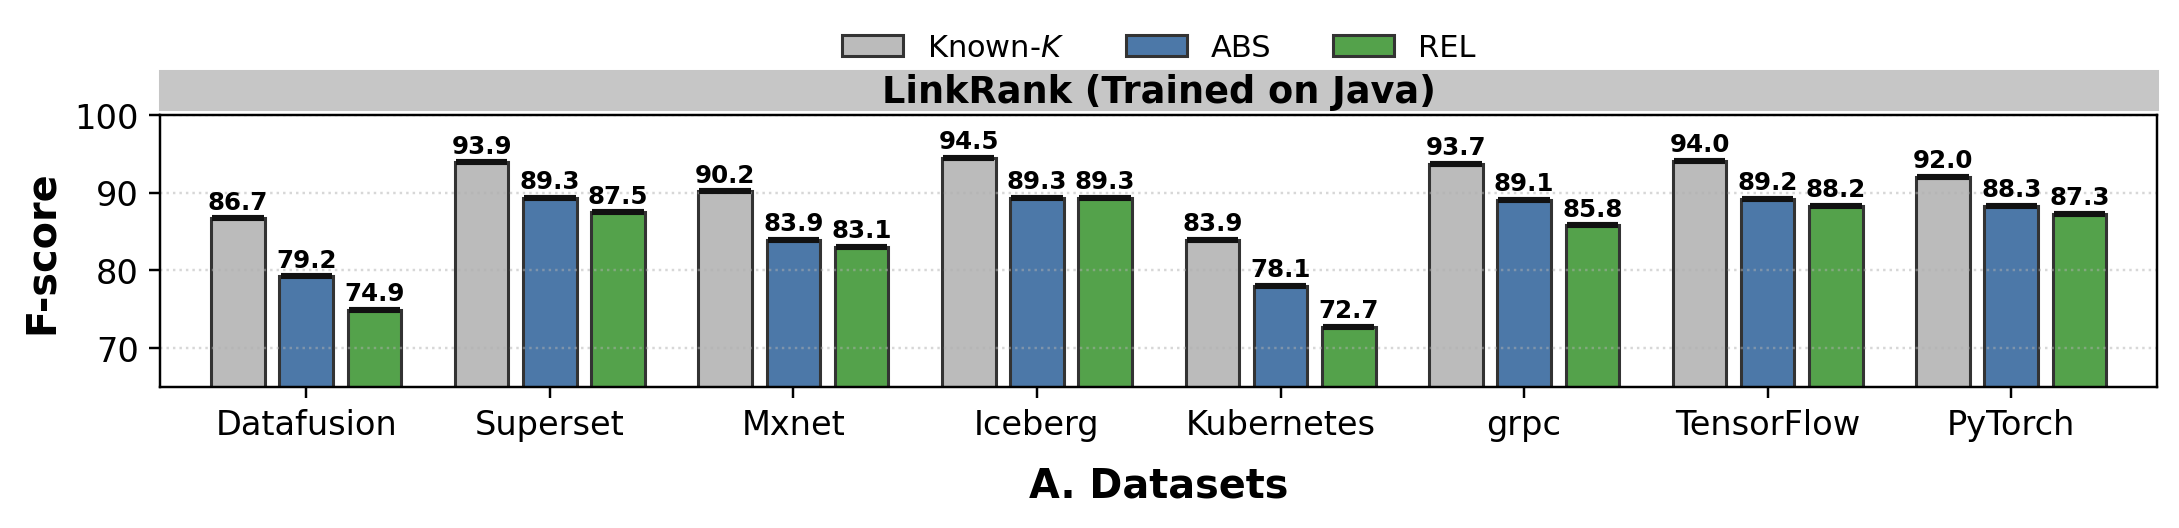
\includegraphics[width=\linewidth]{Figures/LR-java.png}
  \caption{Cross-project performance of \textsc{LinkRank} trained on Java repositories. }
  \subcaption*{Panels show per-dataset F\textsubscript{1} under Known-$K$, ABS, and REL regimes.}
  \label{fig:LR-java}
\end{figure}

\begin{figure}[H]
  \centering
  \includegraphics[width=\linewidth]{Figures/lr-C2I-java.png}
  \caption{Cross-project performance of \textsc{LinkRank-C2I} trained on Java repositories.}
  \label{fig:LR-C2I-java}
\end{figure}


% =======================
%   TRAINED ON RUST & GO
% =======================
\begin{figure}[H]
  \centering
  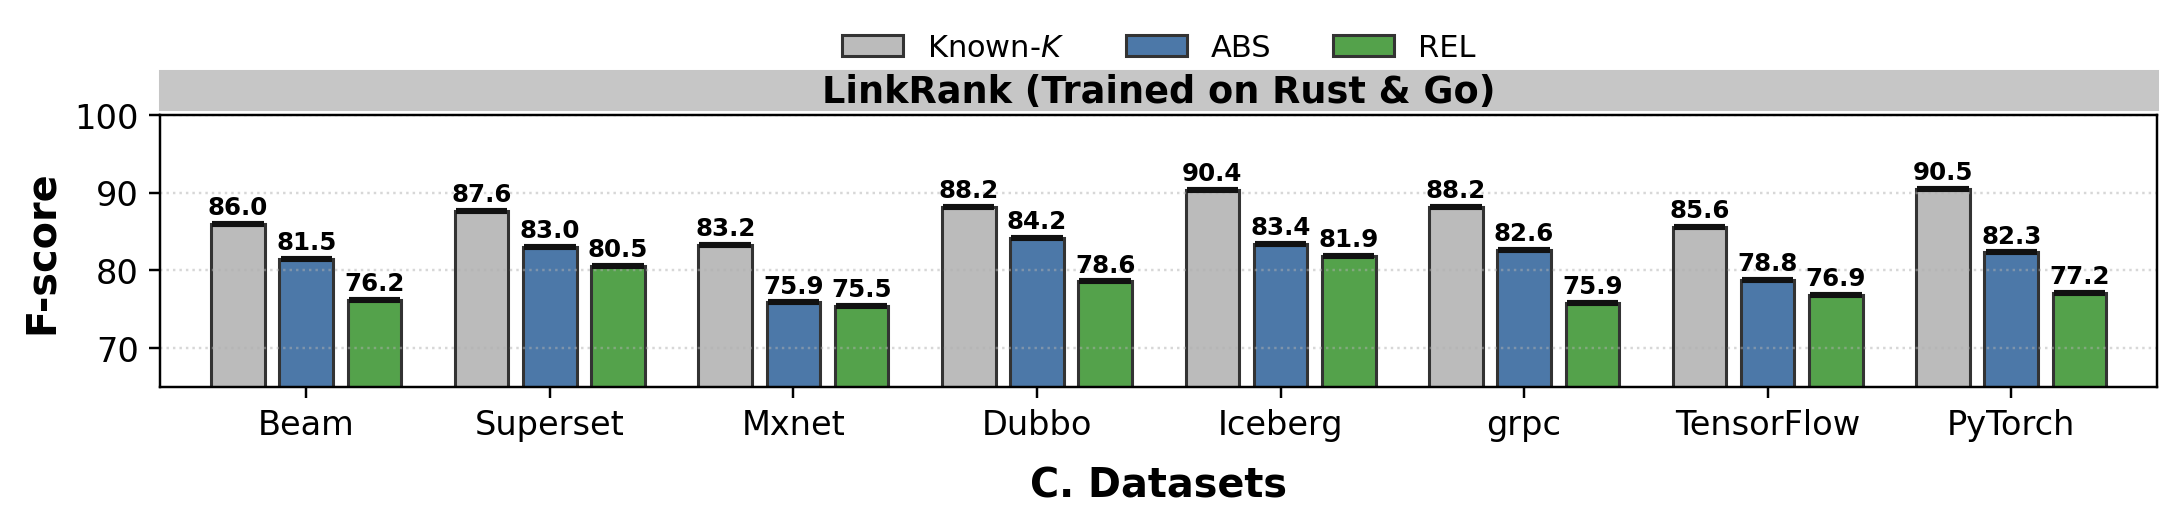
\includegraphics[width=\linewidth]{Figures/LR-rust.png}
  \caption{Cross-project performance of \textsc{LinkRank} trained on Go \& Rust repositories.}
  \label{fig:LR-rust}
\end{figure}

\begin{figure}[H]
  \centering
  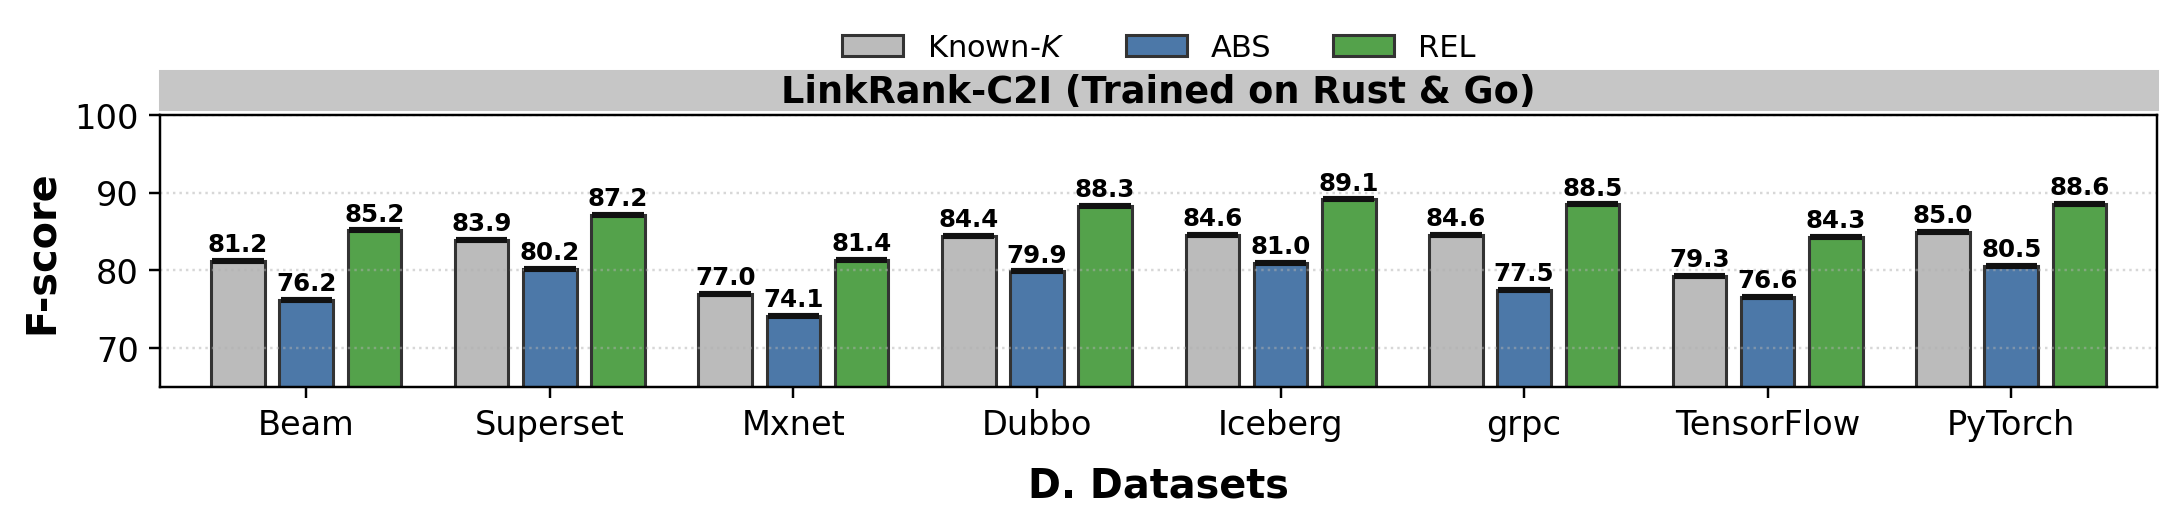
\includegraphics[width=\linewidth]{Figures/LR-C2I-rust.png}
  \caption{Cross-project performance of \textsc{LinkRank-C2I} trained on Go \& Rust repositories.}
  \label{fig:LR-C2I-rust}
\end{figure}


% =======================
%   TRAINED ON C++
% =======================
\begin{figure}[H]
  \centering
  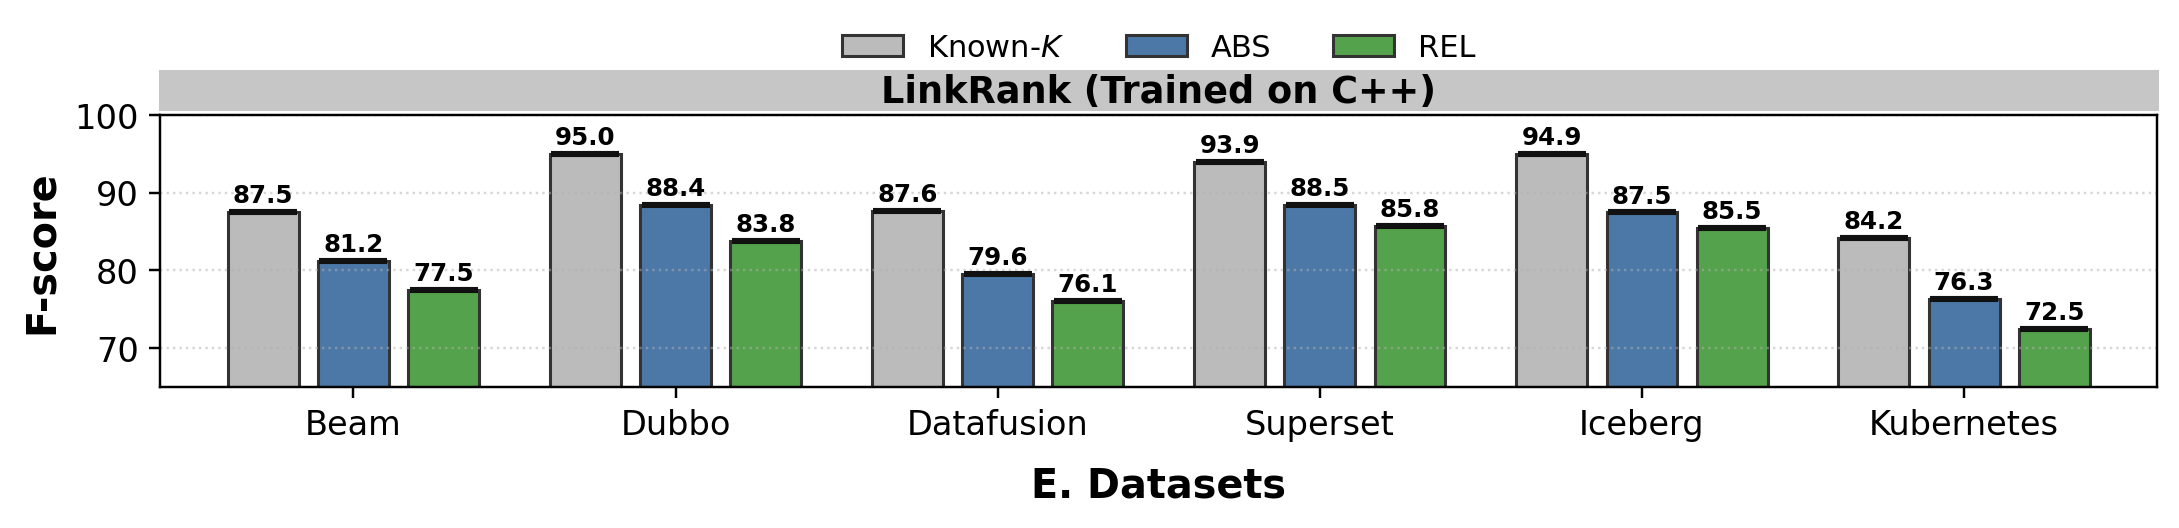
\includegraphics[width=\linewidth]{Figures/LR-cpp.png}
  \caption{Cross-project performance of \textsc{LinkRank} trained on C++ repositories.}
  \label{fig:LR-cpp}
\end{figure}

\begin{figure}[H]
  \centering
  \includegraphics[width=\linewidth]{Figures/lr-C2I-cpp.png}
  \caption{Cross-project performance of \textsc{LinkRank-C2I} trained on C++ repositories.}
  \label{fig:LR-C2I-cpp}
\end{figure}

Figures~\ref{fig:LR-java}--\ref{fig:LR-C2I-cpp} illustrate the cross-repository performance of LinkRank and LinkRank-C2I when trained on Java, Go \& Rust, and C++ repositories, respectively. For our proposed approaches, we observe a moderate performance drop compared to the non-cross-project setting. But considering the challenges of domain shift across programming languages and repository conventions, the models maintain competitive performance.\\


For LinkRank, training on Rust and Go leads to an approximate 5\% decrease in the ABS setting and around 7\% in the REL setting, highlighting the sensitivity of the model to language differences. For LinkRank-C2I, the decline is more pronounced, with about a 10\% drop under the Known-$K$ scenario and roughly 6\% in the ABS setting.  Despite these decreases, both models continue to achieve competitive scores across repositories, showing that our learning-to-rank framework remains effective and robust even in challenging cross-project scenarios.


% =======================
%   BASELINE METHODS
% =======================
\begin{figure}[H]
  \centering
  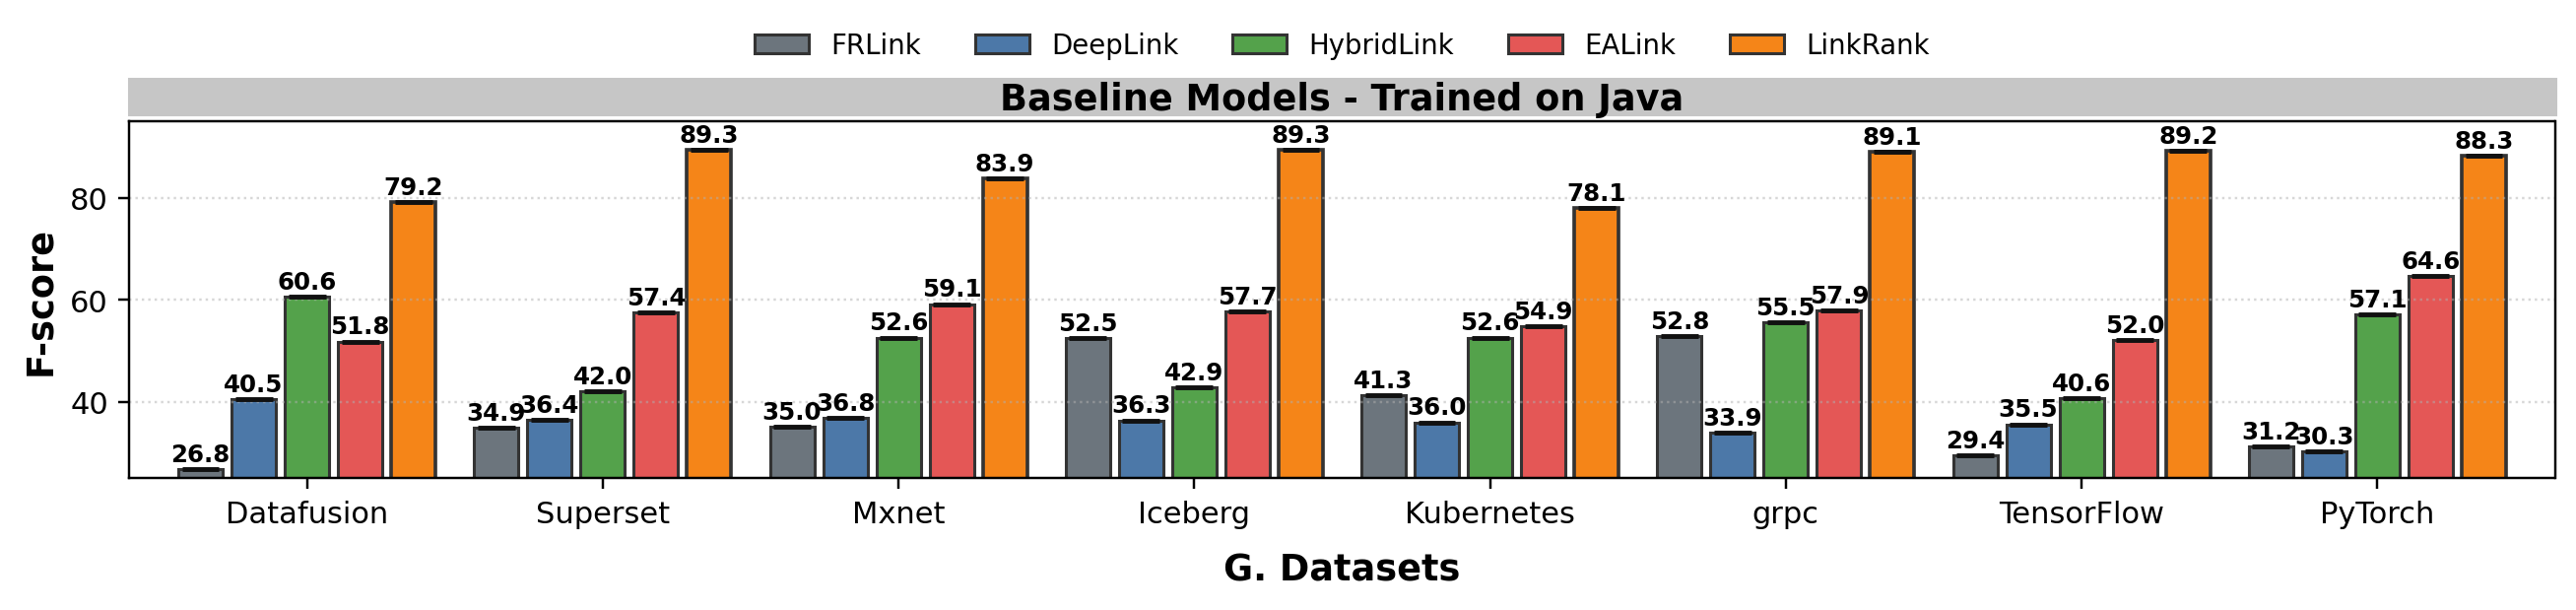
\includegraphics[width=\linewidth]{Figures/baseline_java.png}
  \caption{Baseline performance comparison for Java repositories}
  \subcaption*{(\textsc{FRLink}, \textsc{DeepLink}, \textsc{HybridLinker}, \textsc{EALink})}
  \label{fig:baseline_java}
\end{figure}

\begin{figure}[H]
  \centering
  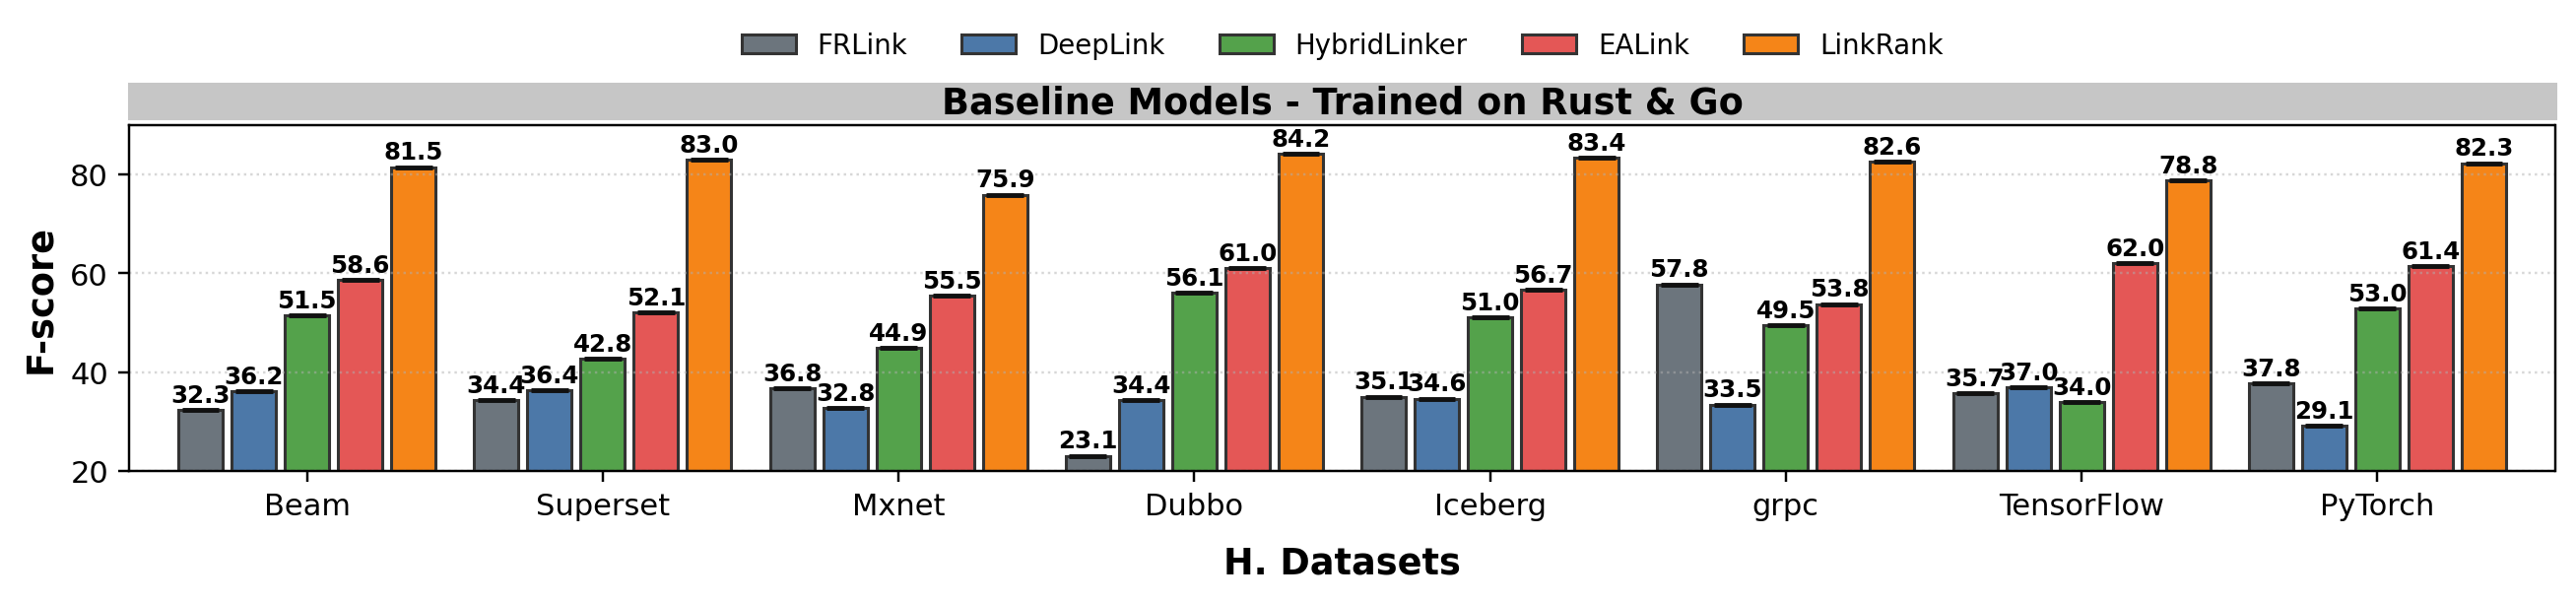
\includegraphics[width=\linewidth]{Figures/baseline_rust_go.png}
  \caption{Baseline performance comparison for Go \& Rust repositories.}
  \label{fig:baseline_rust_go}
\end{figure}

\begin{figure}[H]
  \centering
  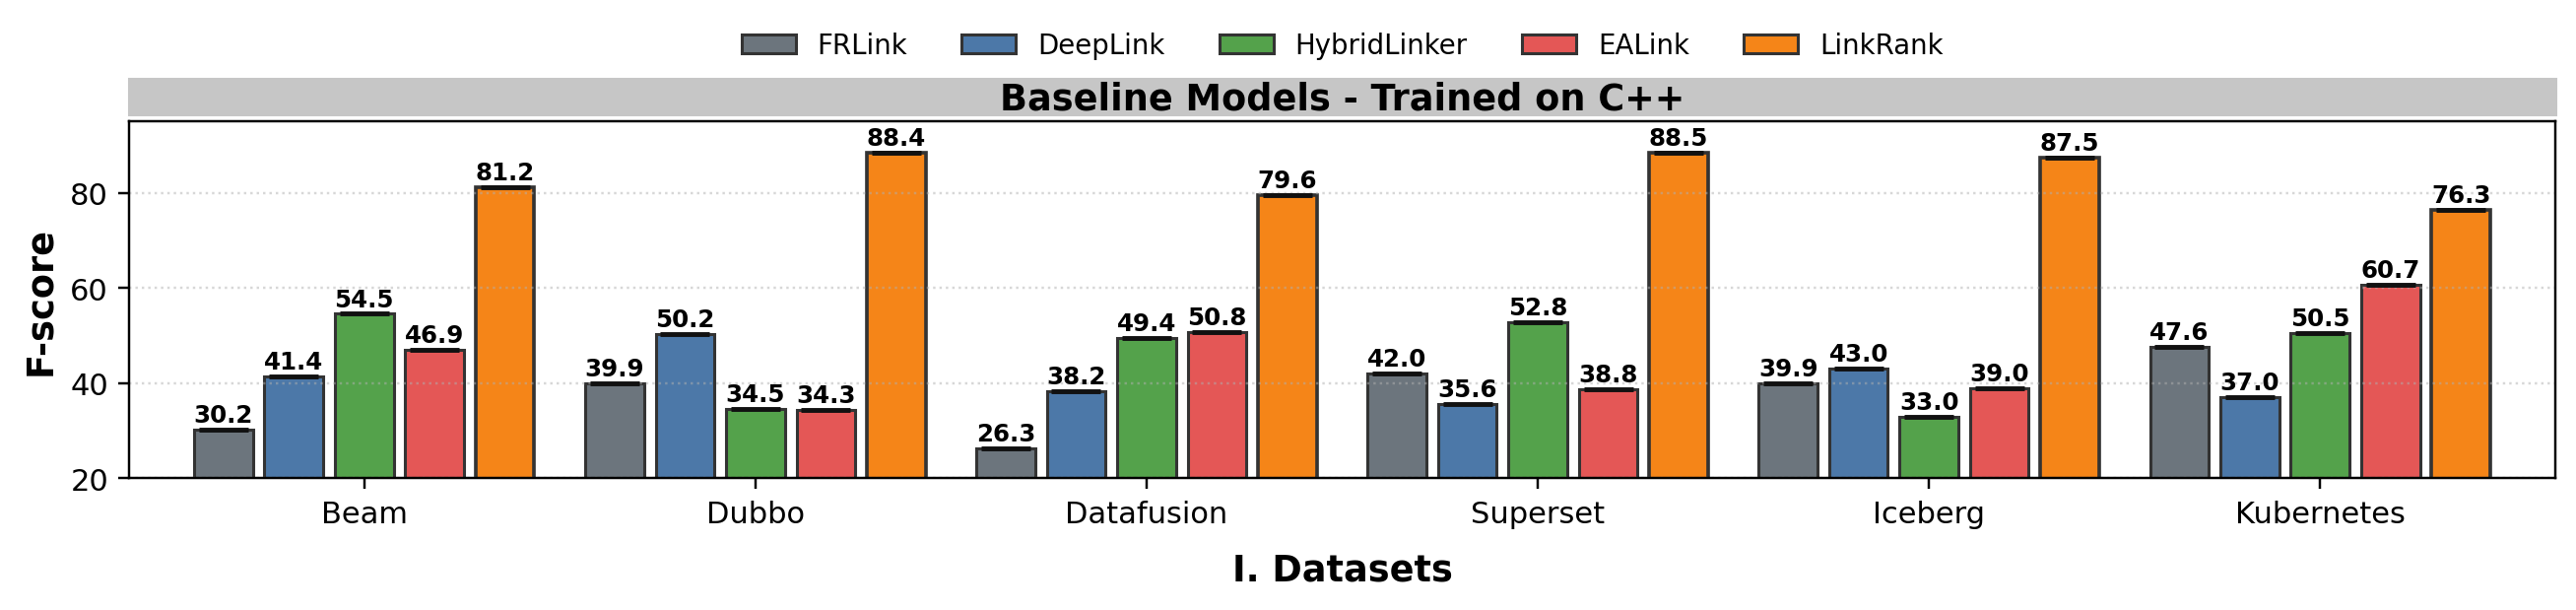
\includegraphics[width=\linewidth]{Figures/baseline_cpp.png}
  \caption{Baseline performance comparison for C++ repositories.}
  \label{fig:baseline_cpp}
\end{figure}

The baseline results can also be seen in the bar plots.  When we compute the average performance drop across all test datasets, FRLink shows the largest degradation, 19.24\% when trained on Rust and Go, and around 18\% when trained on either C++ or Java.  DeepLink drops by 14.27\% (Rust and Go), about 8\% (C++), and 13.51\% (Java).  HybridLinker exhibits 10.9\% (Rust and Go), 13.11\% (C++), and around 8\% (Java).  EALink is comparatively more stable, with about 4\% (Rust and Go), 16.4\% (C++), and 5.47\% (Java).  Taken together, the baselines experience non-trivial but heterogeneous losses under cross-project transfer, with EALink generally the most resilient and FRLink the most sensitive. Overall, we see that LinkRank remains comparatively more stable and effective across language boundaries than the baseline methods.
\section{Conclusion and Future Work}

Modern software maintenance is hampered by the disconnect between issue reports and the corresponding code changes. This thesis presented the vision for an end-to-end, Agentic AI-driven bug resolution system, conceptualized as a three-stage pipeline: \textbf{Traceability} $\rightarrow$ \textbf{Explainability} $\rightarrow$ \textbf{Resolution}. Such a system promises to automate the entire lifecycle of a bug, from identification to a verified fix. However, the efficacy of the entire pipeline is critically dependent on the quality of its foundation: accurately tracing which commits resolve which issues.\\

\noindent
The central challenge, and the primary focus of this thesis, was that existing traceability research has largely overlooked the common and complex reality of \textit{one-to-many} relationships, where a single issue is resolved by multiple, distinct commits. This gap renders most automated tools insufficient for grounding the high-level reasoning required by an intelligent agent.

\subsection*{Summary of Contributions}

This work successfully addressed this foundational problem by designing, implementing, and evaluating \textbf{LinkRank}, a novel learning-to-rank framework specifically engineered for the one-to-many issue-commit recovery task. The key contributions of this thesis are:

\begin{enumerate}
    \item \textbf{A Novel One-to-Many Dataset:} We constructed a new, large-scale dataset from diverse GitHub repositories that explicitly captures genuine one-to-many issue-commit relationships, derived from pull request data. This provides a robust corpus for training and evaluating models on this complex task.

    \item \textbf{The LinkRank Framework:} We formulated issue-commit linking as a ranking problem, a more natural fit for this task than binary classification. LinkRank employs a \textbf{LambdaMART} ranker over a lightweight and effective feature set, combining lexical signals (TF-IDF+SVD) and retrieval-focused matching (BM25).

    \item \textbf{Iterative Selection Strategies:} We introduced practical selection mechanisms (\texttt{Unknown-K ABS} and \texttt{REL}) that allow the model to autonomously determine the complete set of relevant commits for an issue without prior knowledge of the set's size.

    \item \textbf{Comprehensive Evaluation:} Extensive experiments demonstrated that both LinkRank and its bidirectional variant, LinkRank-C2I, \textbf{substantially outperform} existing baseline methods by a large margin (over 25-35 F1 points). Our results also confirmed that the lightweight IR features provide the vast majority of the performance, making LinkRank both effective and computationally efficient.
\end{enumerate}

\subsection*{Future Work: Building the Agentic Pipeline}

This thesis has successfully established the first and most critical pillar of the proposed agentic system. By providing a high-fidelity traceability layer, we have laid the necessary groundwork for the subsequent phases of Explainability and Resolution. Future work will build directly upon the accurate one-to-many links recovered by LinkRank.

    \paragraph{Phase 2: Explainability:} The next logical step is to move from \textit{what} (the links) to \textit{why} (the rationale). We envision a new model, likely a fine-tuned Large Language Model or a similar architecture, that takes an issue description and the complete set of its resolving commits (as identified by LinkRank) as input. Its goal would be to analyze the code diffs in the context of the issue and generate a concise, natural-language explanation of the bug's root cause and the logic of the applied multi-commit solution. The main goal of Explainability is to identify and reason which code changes contribute to which aspects of the issue resolution, thereby providing human-understandable justifications for the automated fixes.

    \paragraph{Phase 3: Resolution:} With a comprehensive understanding of issues, linked commits, and their explanations, the final stage is to build an autonomous resolution agent. This agent would leverage the patterns learned in the first two phases to address new, unseen issues. Given a new bug report, the agent would first retrieve similar explained-and-resolved issues, then reason about the context of the new bug, and finally \textbf{propose candidate code patches} or even a sequence of commits to resolve it. This could involve generating code diffs directly or suggesting modifications to existing code, effectively closing the loop from issue identification to autonomous resolution.

    \paragraph{Full Integration:} The ultimate goal is to integrate all three components---Traceability (LinkRank), Explainability (LLM-based rationale generation), and Resolution (patch generation)---into a single, closed-loop Agentic AI framework. This system would be powerful enough to automatically trigger on new issues, trace the relevant commits, explain the reasoning, and propose fixes with minimal human intervention, revolutionizing the software maintenance landscape.\\


In conclusion, this work has solved a long-standing and critical gap in software traceability. By delivering a robust solution for the one-to-many linking problem, this thesis provides the indispensable foundation required to build the next generation of truly intelligent and autonomous software maintenance agents.

\section{Dissemination}

A.Kumar, T.Mondal, P.P.Das, P.P.Chakrabarti, “LinkRank: A Learning-to-Rank Framework for One-to-Many Issue–Commit Traceability” in IEEE Transactions on Software Engineering (TSE). [Submitted, under review]





\newpage
\bibliographystyle{IEEEtran}
\bibliography{ref}
\end{document}